% Options for packages loaded elsewhere
% Options for packages loaded elsewhere
\PassOptionsToPackage{unicode}{hyperref}
\PassOptionsToPackage{hyphens}{url}
\PassOptionsToPackage{dvipsnames,svgnames,x11names}{xcolor}
%
\documentclass[
  11pt,
  article]{jss}
\usepackage{xcolor}
\usepackage{amsmath,amssymb}
\setcounter{secnumdepth}{-\maxdimen} % remove section numbering
\usepackage{iftex}
\ifPDFTeX
  \usepackage[T1]{fontenc}
  \usepackage[utf8]{inputenc}
  \usepackage{textcomp} % provide euro and other symbols
\else % if luatex or xetex
  \usepackage{unicode-math} % this also loads fontspec
  \defaultfontfeatures{Scale=MatchLowercase}
  \defaultfontfeatures[\rmfamily]{Ligatures=TeX,Scale=1}
\fi
\usepackage{lmodern}
\ifPDFTeX\else
  % xetex/luatex font selection
\fi
% Use upquote if available, for straight quotes in verbatim environments
\IfFileExists{upquote.sty}{\usepackage{upquote}}{}
\IfFileExists{microtype.sty}{% use microtype if available
  \usepackage[]{microtype}
  \UseMicrotypeSet[protrusion]{basicmath} % disable protrusion for tt fonts
}{}
\makeatletter
\@ifundefined{KOMAClassName}{% if non-KOMA class
  \IfFileExists{parskip.sty}{%
    \usepackage{parskip}
  }{% else
    \setlength{\parindent}{0pt}
    \setlength{\parskip}{6pt plus 2pt minus 1pt}}
}{% if KOMA class
  \KOMAoptions{parskip=half}}
\makeatother
% Make \paragraph and \subparagraph free-standing
\makeatletter
\ifx\paragraph\undefined\else
  \let\oldparagraph\paragraph
  \renewcommand{\paragraph}{
    \@ifstar
      \xxxParagraphStar
      \xxxParagraphNoStar
  }
  \newcommand{\xxxParagraphStar}[1]{\oldparagraph*{#1}\mbox{}}
  \newcommand{\xxxParagraphNoStar}[1]{\oldparagraph{#1}\mbox{}}
\fi
\ifx\subparagraph\undefined\else
  \let\oldsubparagraph\subparagraph
  \renewcommand{\subparagraph}{
    \@ifstar
      \xxxSubParagraphStar
      \xxxSubParagraphNoStar
  }
  \newcommand{\xxxSubParagraphStar}[1]{\oldsubparagraph*{#1}\mbox{}}
  \newcommand{\xxxSubParagraphNoStar}[1]{\oldsubparagraph{#1}\mbox{}}
\fi
\makeatother


\usepackage{longtable,booktabs,array}
\usepackage{calc} % for calculating minipage widths
% Correct order of tables after \paragraph or \subparagraph
\usepackage{etoolbox}
\makeatletter
\patchcmd\longtable{\par}{\if@noskipsec\mbox{}\fi\par}{}{}
\makeatother
% Allow footnotes in longtable head/foot
\IfFileExists{footnotehyper.sty}{\usepackage{footnotehyper}}{\usepackage{footnote}}
\makesavenoteenv{longtable}
\usepackage{graphicx}
\makeatletter
\newsavebox\pandoc@box
\newcommand*\pandocbounded[1]{% scales image to fit in text height/width
  \sbox\pandoc@box{#1}%
  \Gscale@div\@tempa{\textheight}{\dimexpr\ht\pandoc@box+\dp\pandoc@box\relax}%
  \Gscale@div\@tempb{\linewidth}{\wd\pandoc@box}%
  \ifdim\@tempb\p@<\@tempa\p@\let\@tempa\@tempb\fi% select the smaller of both
  \ifdim\@tempa\p@<\p@\scalebox{\@tempa}{\usebox\pandoc@box}%
  \else\usebox{\pandoc@box}%
  \fi%
}
% Set default figure placement to htbp
\def\fps@figure{htbp}
\makeatother





\setlength{\emergencystretch}{3em} % prevent overfull lines

\providecommand{\tightlist}{%
  \setlength{\itemsep}{0pt}\setlength{\parskip}{0pt}}





\usepackage{booktabs}
\usepackage{longtable}
\usepackage{array}
\usepackage{multirow}
\usepackage{wrapfig}
\usepackage{float}
\usepackage{pdflscape}
\usepackage{tabu}
\usepackage{threeparttable}
\usepackage{threeparttablex}
\usepackage[normalem]{ulem}
\usepackage[utf8]{inputenc}
\usepackage{makecell}
\usepackage{xcolor}
\usepackage{placeins}
% \usepackage{tcolorbox}
\newtheorem{definition}{Definition}
\renewcommand{\texttt}[1]{\code{#1}}
% \newtcolorbox{mybox}[1]{colback=gray!10, colframe=gray!80, title=#1}
\usepackage{orcidlink,thumbpdf,lmodern}

\newcommand{\class}[1]{`\code{#1}'}
\newcommand{\fct}[1]{\code{#1()}}
\makeatletter
\@ifpackageloaded{tcolorbox}{}{\usepackage[skins,breakable]{tcolorbox}}
\@ifpackageloaded{fontawesome5}{}{\usepackage{fontawesome5}}
\definecolor{quarto-callout-color}{HTML}{909090}
\definecolor{quarto-callout-note-color}{HTML}{0758E5}
\definecolor{quarto-callout-important-color}{HTML}{CC1914}
\definecolor{quarto-callout-warning-color}{HTML}{EB9113}
\definecolor{quarto-callout-tip-color}{HTML}{00A047}
\definecolor{quarto-callout-caution-color}{HTML}{FC5300}
\definecolor{quarto-callout-color-frame}{HTML}{acacac}
\definecolor{quarto-callout-note-color-frame}{HTML}{4582ec}
\definecolor{quarto-callout-important-color-frame}{HTML}{d9534f}
\definecolor{quarto-callout-warning-color-frame}{HTML}{f0ad4e}
\definecolor{quarto-callout-tip-color-frame}{HTML}{02b875}
\definecolor{quarto-callout-caution-color-frame}{HTML}{fd7e14}
\makeatother
\makeatletter
\@ifpackageloaded{caption}{}{\usepackage{caption}}
\AtBeginDocument{%
\ifdefined\contentsname
  \renewcommand*\contentsname{Table of contents}
\else
  \newcommand\contentsname{Table of contents}
\fi
\ifdefined\listfigurename
  \renewcommand*\listfigurename{List of Figures}
\else
  \newcommand\listfigurename{List of Figures}
\fi
\ifdefined\listtablename
  \renewcommand*\listtablename{List of Tables}
\else
  \newcommand\listtablename{List of Tables}
\fi
\ifdefined\figurename
  \renewcommand*\figurename{Figure}
\else
  \newcommand\figurename{Figure}
\fi
\ifdefined\tablename
  \renewcommand*\tablename{Table}
\else
  \newcommand\tablename{Table}
\fi
}
\@ifpackageloaded{float}{}{\usepackage{float}}
\floatstyle{ruled}
\@ifundefined{c@chapter}{\newfloat{codelisting}{h}{lop}}{\newfloat{codelisting}{h}{lop}[chapter]}
\floatname{codelisting}{Listing}
\newcommand*\listoflistings{\listof{codelisting}{List of Listings}}
\makeatother
\makeatletter
\makeatother
\makeatletter
\@ifpackageloaded{caption}{}{\usepackage{caption}}
\@ifpackageloaded{subcaption}{}{\usepackage{subcaption}}
\makeatother
\makeatletter
\@ifpackageloaded{tcolorbox}{}{\usepackage[skins,breakable]{tcolorbox}}
\makeatother
\makeatletter
\@ifundefined{shadecolor}{\definecolor{shadecolor}{rgb}{.97, .97, .97}}{}
\makeatother
\makeatletter
\makeatother
\makeatletter
\ifdefined\Shaded\renewenvironment{Shaded}{\begin{tcolorbox}[boxrule=0pt, borderline west={3pt}{0pt}{shadecolor}, breakable, sharp corners, interior hidden, frame hidden, enhanced]}{\end{tcolorbox}}\fi
\makeatother
\usepackage{bookmark}
\IfFileExists{xurl.sty}{\usepackage{xurl}}{} % add URL line breaks if available
\urlstyle{same}
\hypersetup{
  pdftitle={Making, Updating, and Querying Causal Models with },
  pdfauthor={Till Tietz; Lily Medina; Georgiy Syunyaev; Macartan Humphreys},
  colorlinks=true,
  linkcolor={blue},
  filecolor={Maroon},
  citecolor={Blue},
  urlcolor={Blue},
  pdfcreator={LaTeX via pandoc}}


%% -- Article metainformation (author, title, ...) -----------------------------

%% Author information
\author{Till Tietz~\orcidlink{0000-0002-2916-9059}\\Humboldt
University \And Lily Medina~\orcidlink{0009-0004-2423-524X}\\University
of California, Berkeley \AND Georgiy
Syunyaev~\orcidlink{0000-0002-4391-6313}\\Vanderbilt
University \And Macartan Humphreys~\orcidlink{0000-0001-7029-2326}\\WZB}
\Plainauthor{Till Tietz, Lily Medina, Georgiy Syunyaev, Macartan
Humphreys} %% comma-separated

\title{Making, Updating, and Querying Causal Models with
\pkg{CausalQueries}}
\Plaintitle{Making, Updating, and Querying Causal Models
with} %% without formatting

%% an abstract and keywords
\Abstract{The \proglang{R} package \pkg{CausalQueries} can be used to
make, update, and query causal models defined on binary nodes. Users
provide a causal statement of the form
\texttt{X\ -\textgreater{}\ M\ \textless{}-\ Y;\ M\ \textless{}-\textgreater{}\ Y}
which is interpreted as a structural causal model over a collection of
binary nodes. Then \pkg{CausalQueries} allows users to (1) identify the
set of principal strata---causal types---required to characterize all
possible causal relations between nodes that are consistent with the
causal statement (2) determine a set of parameters needed to
characterize distributions over these causal types (3) update beliefs
over distributions of causal types, using a \texttt{stan} model plus
data, and (4) pose a wide range of causal queries of the model, using
either the prior distribution, the posterior distribution, or a
user-specified candidate vector of parameters.}

%% at least one keyword must be supplied
\Keywords{causal model, Bayesian updating, DAG, Stan}

%% publication information
%% NOTE: Typically, this can be left commented and will be filled out by the technical editor
%% \Volume{50}
%% \Issue{9}
%% \Month{June}
%% \Year{2012}
%% \Submitdate{2012-06-04}
%% \Acceptdate{2012-06-04}
%% \setcounter{page}{1}
%% \Pages{1--xx}

%% The address of (at least) one author should be given
%% in the following format:
\Address{
Till Tietz\\
Humboldt University\\
Berlin Germany\\
E-mail: \email{ttietz2014@gmail.com}\\
URL: \url{https://github.com/till-tietz}\\
\\~
Lily Medina\\
University of California, Berkeley\\
E-mail: \email{lily.medina@berkeley.edu}\\
URL: \url{https://lilymedina.github.io/}\\
\\~
Georgiy Syunyaev\\
Vanderbilt University\\
E-mail: \email{g.syunyaev@vanderbilt.edu}\\
URL: \url{https://gsyunyaev.com/}\\
\\~
Macartan Humphreys\\
WZB, IPI\\
Reichpietschufer 50\\
Berlin Germany\\
E-mail: \email{macartan.humphreys@wzb.eu}\\
URL: \url{https://macartan.github.io/}\\
\\~

}

\begin{document}
\maketitle


\section{Introduction: Causal models}\label{sec-intro}

\pkg{CausalQueries} is an \proglang{R} package that lets users make,
update, and query causal models. Users provide a structural causal model
in the form of a statement that reports a set of binary variables and
the relations of causal ancestry between them. There are three primary
functions. The first, \texttt{make\_model()}, takes a causal statement
and generates a parameter vector that fully describes a probability
distribution over all possible types of causal relations between
variables (``causal types''). Given a prior distribution over
parameters---equivalently, over causal models consistent with the
structural model--- and data on some or all nodes, the second primary
function, \texttt{update\_model()}, deploys a Stan
\citep{carpenter_stan_2017} model to generate a posterior distribution
over causal models. The third primary function \texttt{query\_model()}
can then be used to ask a wide range of causal queries, using either the
prior distribution, the posterior distribution, or a user-specified
candidate vector of parameters.

In the next section we provide a motivating example that uses the three
primary functions together. We then describe how the package relates to
existing available software. Section~\ref{sec-theory} gives an overview
of the statistical model behind the package. Section~\ref{sec-make},
Section~\ref{sec-update}, and Section~\ref{sec-query} then describe, in
turn, the functionality for making, updating, and querying causal
models. We provide further computation details in the final section.

\section{Motivating example}\label{motivating-example}

Before providing details on package functionality, we give an example of
an application of the three primary functions, showing how to use
\pkg{CausalQueries} to replicate the analysis in
\citetext{\citealp{chickering_clinicians_1996}; \citealp[see
also][]{humphreys_integrated_2023}}.

\citet{chickering_clinicians_1996} seek to draw inferences on causal
effects in the presence of imperfect compliance. We have access to an
instrument \(Z\) (a randomly assigned prescription for cholesterol
medication), which is a cause of \(X\) (treatment uptake) but otherwise
unrelated to \(Y\) (cholesterol). We imagine we are interested in three
specific queries. The first is the average causal effect of \(X\) on
\(Y\). The second is the average effect for units for which \(X=0\) and
\(Y=0\); this ``probability of causation'' query asks whether untreated
individuals with bad outcomes did poorly \emph{because} they were
untreated. The last is the average effect for ``compliers'': units for
which \(X\) responds positively to \(Z\). Thus two of these queries are
conditional queries, with one conditional on a counterfactual quantity.

The data on \(Z\), \(X\), and \(Y\) is given in
\citet{chickering_clinicians_1996} and is also included in the
\pkg{CausalQueries} package. The data looks as follows:

\begin{CodeInput}
R> data("lipids_data")
R> lipids_data
\end{CodeInput}

\begin{verbatim}
   event strategy count
1 Z0X0Y0      ZXY   158
2 Z1X0Y0      ZXY    52
3 Z0X1Y0      ZXY     0
4 Z1X1Y0      ZXY    23
5 Z0X0Y1      ZXY    14
6 Z1X0Y1      ZXY    12
7 Z0X1Y1      ZXY     0
8 Z1X1Y1      ZXY    78
\end{verbatim}

This data is reported in ``compact form,'' meaning it records the number
of units (``count'') that display each possible pattern of outcomes on
\(Z\), \(X\), and \(Y\) (``event'').

The strategy to analyse this data involves three steps:

\begin{itemize}
\tightlist
\item
  Step 1: generate a model with \texttt{make\_model}, yielding an object
  of class \texttt{causal\_model},
\item
  Step 2: update the model with \texttt{update\_model}, again yielding
  an object of class \texttt{causal\_model},
\item
  Step 3: pose queries of the model with \texttt{query\_model}, yielding
  an object of class \texttt{model\_query}.
\end{itemize}

Users generate the stipulated causal model using \pkg{CausalQueries} as
follows:

\begin{CodeInput}
R> lipids_model <-  make_model("Z -> X -> Y; X <-> Y") 
\end{CodeInput}

The result is an object of class \texttt{causal\_model}, with associated
\texttt{print}, \texttt{summary}, and \texttt{plot} methods. By default,
uniform priors are placed on model parameters.

Users can then \emph{update} beliefs over model parameters by supplying
data as follows:

\begin{CodeInput}
R> lipids_model <- update_model(lipids_model, lipids_data)
\end{CodeInput}

The updated model is also an object of class \texttt{causal\_model},
though now also containing a posterior distribution over model
parameters.

Finally, users can \emph{query} the model. For instance, the three
previously mentioned queries, which vary in the type of conditioning
imposed, can be formulated as follows:

\begin{CodeInput}
R> lipids_queries <- query_model(lipids_model, queries = list(
+    ATE = "Y[X = 1] - Y[X = 0]",
+    PoC = "Y[X = 1] - Y[X = 0] :|: X == 0 & Y == 0",
+    LATE = "Y[X = 1] - Y[X = 0] :|: X[Z = 1] > X[Z = 0]"),
+    using = "posteriors")
\end{CodeInput}

The output is an object of class \texttt{model\_query}, with associated
\texttt{print}, \texttt{summary}, and \texttt{plot} methods.

The \texttt{model\_query} object is a data frame containing estimates,
and, when available, prior or posterior standard deviations, and
credibility intervals.

Table~\ref{tbl-lipids} presents the results from the analysis of the
lipids data.\footnote{Note that the ``using'' column is omitted to
  simplify output, as all estimands are derived from the posterior
  distribution.} Rows 1 and 2 in the table replicate the results from
\citet{chickering_clinicians_1996}, while row 3 provides inferences for
the local average treatment effects (LATE).

\begin{longtable}{ccccccc}

\toprule
label & query & given & mean & sd & cred.low & cred.high\\
\midrule
ATE & Y[X = 1] - Y[X = 0] & - & 0.55 & 0.10 & 0.37 & 0.73\\
PoC & Y[X = 1] - Y[X = 0] & X == 0 \& Y == 0 & 0.64 & 0.15 & 0.37 & 0.89\\
LATE & Y[X = 1] - Y[X = 0] & X[Z = 1] > X[Z = 0] & 0.70 & 0.05 & 0.59 & 0.80\\
\bottomrule


\caption{\label{tbl-lipids}Replication of
\citet{chickering_clinicians_1996}.}

\tabularnewline
\end{longtable}

For visual presentation of the results, output can also be plotted:

\begin{CodeInput}
R> lipids_queries |> plot()
\end{CodeInput}

\begin{figure}[H]

{\centering \pandocbounded{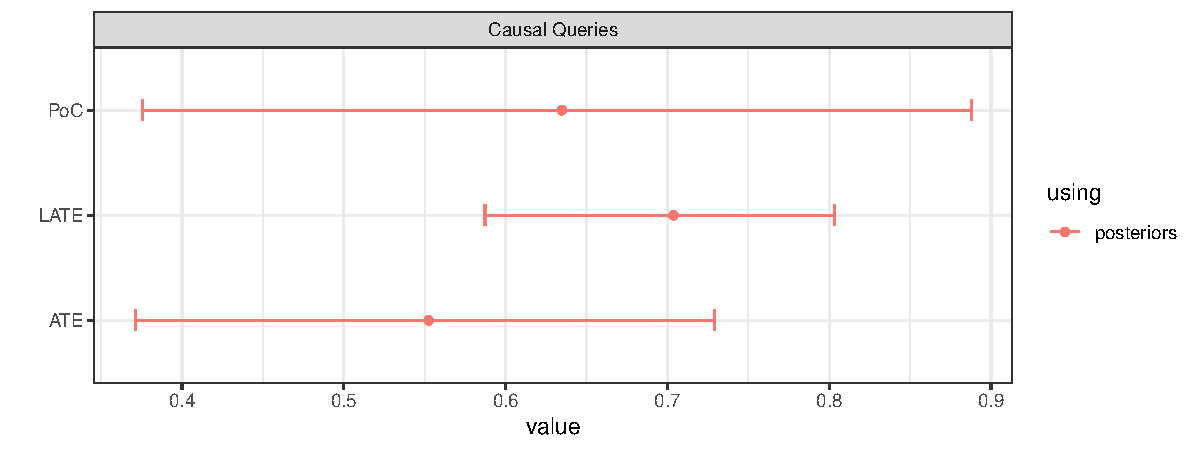
\includegraphics[keepaspectratio]{paper_files/figure-pdf/queryplot-1.pdf}}

}

\caption{Illustration of queries plotted.}

\end{figure}%

These core functions can be combined in a single pipeline as follows:

\begin{CodeInput}
R> make_model("Z -> X -> Y; X <-> Y") |> update_model(lipids_data) |>
+    query_model(queries = list(ATE = "Y[X = 1] - Y[X = 0]",
+    PoC  = "Y[X = 1] - Y[X = 0] :|: X == 0 & Y == 0",
+    LATE = "Y[X = 1] - Y[X = 0] :|: X[Z = 1] > X[Z = 0]"),
+    using = "posteriors") |> plot()
\end{CodeInput}

As we describe below, the same basic procedure of making, updating, and
querying models, can be used (up to computational constraints) for
arbitrary causal models, for different types of data structures, and for
all causal queries that can be posed of the causal model.

\section{Connections to existing
packages}\label{connections-to-existing-packages}

The field of causal inference encompasses a wide range of software tools
used across various disciplines, including social sciences, natural
sciences, computer science, and applied mathematics. This section
focuses on the role and capabilities of \pkg{CausalQueries} within the
specific area of evaluating causal queries on models represented as
directed acyclic graphs (DAGs) or structural equation models (SEMs).
Table~\ref{tbl-software} provides a summary of relevant software,
highlighting their connections, strengths, and limitations in comparison
to \pkg{CausalQueries}.

\begin{longtable}[]{@{}
  >{\raggedright\arraybackslash}p{(\linewidth - 8\tabcolsep) * \real{0.1800}}
  >{\raggedright\arraybackslash}p{(\linewidth - 8\tabcolsep) * \real{0.1900}}
  >{\raggedright\arraybackslash}p{(\linewidth - 8\tabcolsep) * \real{0.1000}}
  >{\raggedright\arraybackslash}p{(\linewidth - 8\tabcolsep) * \real{0.1700}}
  >{\raggedright\arraybackslash}p{(\linewidth - 8\tabcolsep) * \real{0.3600}}@{}}
\toprule\noalign{}
\begin{minipage}[b]{\linewidth}\raggedright
Software
\end{minipage} & \begin{minipage}[b]{\linewidth}\raggedright
Source
\end{minipage} & \begin{minipage}[b]{\linewidth}\raggedright
Language
\end{minipage} & \begin{minipage}[b]{\linewidth}\raggedright
Availability
\end{minipage} & \begin{minipage}[b]{\linewidth}\raggedright
Scope
\end{minipage} \\
\midrule\noalign{}
\endfirsthead
\toprule\noalign{}
\begin{minipage}[b]{\linewidth}\raggedright
Software
\end{minipage} & \begin{minipage}[b]{\linewidth}\raggedright
Source
\end{minipage} & \begin{minipage}[b]{\linewidth}\raggedright
Language
\end{minipage} & \begin{minipage}[b]{\linewidth}\raggedright
Availability
\end{minipage} & \begin{minipage}[b]{\linewidth}\raggedright
Scope
\end{minipage} \\
\midrule\noalign{}
\endhead
\bottomrule\noalign{}
\tabularnewline
\caption{Related software.}\label{tbl-software}\tabularnewline
\endlastfoot
\pkg{causalnex} & \citet{beaumont_causalnex_2021} & \proglang{Python} &
\begin{minipage}[t]{\linewidth}\raggedright
\begin{itemize}
\tightlist
\item
  pip
\end{itemize}
\end{minipage} & \begin{minipage}[t]{\linewidth}\raggedright
\begin{itemize}
\tightlist
\item
  causal structure learning
\item
  querying marginal distributions
\item
  discrete data
\end{itemize}
\end{minipage} \\
\pkg{pclag} & \citet{kalisch_causal_2012} & \proglang{R} &
\begin{minipage}[t]{\linewidth}\raggedright
\begin{itemize}
\tightlist
\item
  CRAN
\item
  GitHub
\end{itemize}
\end{minipage} & \begin{minipage}[t]{\linewidth}\raggedright
\begin{itemize}
\tightlist
\item
  causal structure learning
\item
  ATEs under linear conditional expectations, no hidden selection
\end{itemize}
\end{minipage} \\
\pkg{DoWhy} & \citet{dowhy} & \proglang{Python} &
\begin{minipage}[t]{\linewidth}\raggedright
\begin{itemize}
\tightlist
\item
  pip
\end{itemize}
\end{minipage} & \begin{minipage}[t]{\linewidth}\raggedright
\begin{itemize}
\tightlist
\item
  identification
\item
  average and conditional causal effects
\item
  robustness checks
\end{itemize}
\end{minipage} \\
\pkg{autobounds} & \citet{duarte_automated_2023} & \proglang{Python} &
\begin{minipage}[t]{\linewidth}\raggedright
\begin{itemize}
\tightlist
\item
  Docker
\item
  GitHub
\end{itemize}
\end{minipage} & \begin{minipage}[t]{\linewidth}\raggedright
\begin{itemize}
\tightlist
\item
  bounding causal effects
\item
  partial identification
\item
  DAG canonicalization
\item
  binary data
\end{itemize}
\end{minipage} \\
\pkg{causaloptim} & \citet{sachs_general_2023} & \proglang{R} &
\begin{minipage}[t]{\linewidth}\raggedright
\begin{itemize}
\tightlist
\item
  CRAN
\item
  GitHub
\end{itemize}
\end{minipage} & \begin{minipage}[t]{\linewidth}\raggedright
\begin{itemize}
\tightlist
\item
  bounding causal effects
\item
  non-identified queries
\item
  binary data
\end{itemize}
\end{minipage} \\
\end{longtable}

\pkg{causalnex} is comprehensive software that offers functions for
discovering and querying causal models. Like \pkg{CausalQueries}, it
uses Bayesian methods and supports ``\texttt{do} calculus''
\citep{pearl_causality_2009}. It focuses on conditional probability
distribution tables instead of principal strata (causal types). This
limits the types of queries and expert information that can be
incorporated. For example, knowing conditional probability distributions
is not enough to make claims about (or provide priors with respect to)
effect monotonicity, complier effects, or the ``probability of
causation'' \citep{dawid2017probability}. However, it allows for
efficient handling of simple queries with larger models.

Similar to \pkg{causalnex}, \pkg{pclag} emphasizes learning about causal
structures and uses the resulting DAGs to recover average treatment
effects (ATEs) across all learned Markov-equivalent classes from
observed data that satisfy linearity of conditional expectations. This
approach is also more restrictive than \pkg{CausalQueries} in terms of
the queries it allows.

\pkg{DoWhy} is a feature-rich framework focusing on causal
identification, effect estimation, and assumption validation. With a
user-specified DAG, it uses do-calculus to find expressions that
identify desired causal effects through Back-door, Front-door,
instrumental variable (IV), and mediation criteria, and then uses
standard estimators to estimate the desired effect. After estimation,
\pkg{DoWhy} deploys a comprehensive refutation engine with a large set
of robustness tests. While this approach efficiently handles varied data
types on large causal models, not parameterizing the DAG itself limits
the types of queries that can be posed.

The packages most similar to \pkg{CausalQueries} for model definition
are \pkg{autobounds} and \pkg{causaloptim}. They deal with discrete
causal models, and their definitions of principal strata (causal types)
and causal relations on the DAG are very similar to those of
\pkg{CausalQueries}. Differences arise in how disturbance terms and
confounding are defined: implicitly by the causal statement in
\pkg{CausalQueries} versus explicitly via separate disturbance nodes in
\pkg{autobounds} and \pkg{causaloptim}. While \pkg{CausalQueries}
assumes a canonical form for input DAGs, \pkg{autobounds} and
\pkg{causaloptim} facilitate canonicalization. The main difference
between the methods is in their approach to evaluating queries.

Both \pkg{autobounds} and \pkg{causaloptim} build on seminal approaches
in \citet{balke_bounds_1997} to construct bounds on queries, using
constrained polynomial and linear optimization, respectively. In
contrast, \pkg{CausalQueries} uses Bayesian inference to generate a
posterior over the causal model, which is then queried \citep[consistent
with][]{chickering_clinicians_1996, zhang_partial_2022}. A key
difference is the target of inference. The polynomial and linear
programming approach is suited to handling larger causal models.
However, due to their similar model parameterization, \pkg{autobounds},
\pkg{causaloptim}, and \pkg{CausalQueries} face similar constraints as
parameter spaces expand rapidly with model size. The Bayesian approach
to model updating and querying is more efficient because a model can be
updated once and queried multiple times, while expensive optimization
runs are needed for each separate query in \pkg{autobounds} and
\pkg{causaloptim}.

In summary, the main strength of \pkg{CausalQueries} is its ability to
let users define an arbitrary DAG and pose any queries on it, using a
canonical procedure to form Bayesian posteriors for those queries,
regardless of whether they are identified. For instance, if researchers
want to learn about the local average treatment effect and their model
meets the conditions in \citet{angrist_identification_1996}, updating
will recover valid estimates as data grows, even if researchers are
unaware that the local average treatment effect is identified or
unfamiliar with the specific estimation method proposed by
\citet{angrist_identification_1996}.

There are two main limitations of the models that \pkg{CausalQueries}
can handle. First, \pkg{CausalQueries} is designed for models with a
relatively small number of binary nodes. Since it does not limit the
range of possible causal relationships in a model, the parameter space
expands quickly with the model's complexity. This complexity growth
depends on the causal structure and increases rapidly with the number of
parents influencing a child node. A chain model like
\(A \rightarrow B \rightarrow C \rightarrow D \rightarrow E\) has only
18 parameters (\(2^1 + 4\times 2^2\)), while a model in which
\(A, B, C, D\) are all direct ancestors of \(E\) has \(65,544\)
parameters (\(4\times 2^1 + 2^{(2^4)}\)). Switching from binary to
nonbinary nodes has similar effects. The restriction to binary nodes is
for computational, not conceptual, reasons.\footnote{See Section 9.4.1
  of \citet{humphreys_integrated_2023} for a method that represents
  non-binary data as a profile of outcomes on multiple binary nodes.}

Second, the package is designed for learning about populations from
independently sampled units. Therefore, it does not inherently address
issues of clustering, hierarchical structures, or purposive sampling.
However, the broader framework can be adapted for these purposes
\citep[see Section 9.4 of][]{humphreys_integrated_2023}. The targets of
inference are case-level or population-level quantities;
\pkg{CausalQueries} is not well-suited for estimating sample quantities.

\section{Statistical model}\label{sec-theory}

The core conceptual framework used by \pkg{CausalQueries} is that
described in Pearl's \emph{Causality} \citep{pearl_causality_2009}.

The two key steps to defining a causal model are to define a causal
structure and then place a probability distribution over the exogeneous
variables in the model.

Relying on ideas in \citeauthor{pearl_causality_2009}
\citetext{\citeyear{pearl_causality_2009}; \citealp[with notation
from][]{humphreys_integrated_2023}}, we define a causal model as
follows:

\begin{definition}
  
  A ``\textbf{causal model}'' is:
  \begin{enumerate}
    \item an ordered collection of ``endogenous nodes" $Y = \{Y_1, Y_2, \dots, Y_n\}$,
    \item an ordered collection of ``exogenous nodes" $\Theta = \{\theta^{Y_1}, \theta^{Y_2}, \dots, \theta^{Y_n}\}$,
    \item an ordered collection of functions $F = \{f_{Y_1}, f_{Y_2}, \dots, f_{Y_n}\}$ with $f_{Y_j}$ specifying, for each $j$, how outcome $Y_j$ depends on $\theta_j$ and realizations of endogenous nodes prior to $Y_j$,
    \item a probability distribution, $\lambda$, over $\Theta$.
  \end{enumerate}
  
\end{definition}

Elements 1-3 define a ``\textbf{structural causal model}.'' These
components pin down a causal structure, specifying which endogenous
nodes are (possible) direct causes of a node, \(Y_j\), given the other
nodes in a model. Such nodes are referred to as the ``parents'' of
\(Y_j\), denoted as \(PA_j\) (where uppercase \(PA_j\) represents the
collection of nodes, and lowercase \(pa_j\) represents a specific set of
values these nodes might assume).

Specifying a structural causal model involves making possibly strong
assumptions, for example about which nodes are not plausibly causes of
other nodes. Even still, without information on the distribution of
exogenous nodes, a structural causal model is generally not rich enough
to allow us to make probabilistic statements about the distribution of
outcomes. Adding the final element of the definition then gives us the
fully specified causal model.

With discrete-valued nodes, it is possible to identify all potential
responses of a node to its parents, which we call ``nodal types''
(``response functions'' in \citet{pearl_causality_2009}). If a node
\(i\) can take on \(k_i\) possible values, then the set of possible
values that the parents of \(j\) can assume is
\(m_j :=\prod_{i\in PA_j}k_i\). Consequently, there are \(k_j^{m_j}\)
different ways that node \(j\) might respond to its parents. For binary
nodes, this simplifies to \(2^{\left(2^{|PA_j|}\right)}\). Thus, an
endogenous node with no parents has 2 nodal types; a binary node with
one binary parent has four types; and a binary node with two parents has
16 types, and so forth.

As a practical matter we need to label response types. In
\pkg{CausalQueries} this is done using subscripts that indicate the
response given different combinations of parents. A node, \(Y\), with
one binary parent, \(X\), has a nodal types subscripted with two values
indicating the two possible values of \(Y\)'s parent (0 or 1):
\((\theta_{00}, \theta_{01}, \theta_{10}, \theta_{11})\), where
\(\theta_{ab}\) labels nodal type \((Y(X=0) = a,Y(X=1) = b)\). The same
approach is used for nodes with more (or fewer) nodal types, where the
\(i\)th digit in the subscript corresponding to the value the node takes
when the parents take on the \(i\)th combination of possible parent
values (listed in colexicographic binary order given the specified
ordering of parents).\footnote{A similar approach may be used for non
  binary nodes though in this case the index components can take on more
  values and then length of indices adjust to reflect the set of all
  possible parent value combinations.}

The complete set of possible causal reactions of a given unit to all
possible values of its parents is represented by its collection of nodal
types at each node. We refer to this collection as a unit's ``causal
type,'' denoted as \(\theta\). These causal types correspond to the
principal strata, which are familiar from the study of instrumental
variables \citep{frangakis_principal_2002}.

\pkg{CausalQueries} treats the set of nodal types of \(Y_j\) as the
domain of exogenous nodes \(\theta^{Y_j}\). The function \(f_{Y_j}\)
then determines the value of \(y\) by simply reporting the value of
\(Y_j\) implied by the nodal type and the values of the parents of
\(Y_j\). Therefore, if \(\theta^{Y_j}_{pa_j}\) is the value for \(j\)
when parents have values \(pa_j\), then
\(f_{Y_j}(\theta^{j}, pa_j) = \theta^{Y_j}_{pa_j}\). Practically, this
means that, given the causal structure, learning about the model reduces
to learning about the distribution, \(\lambda\), over the nodal types.

In scenarios without unobserved confounding, we assume that the
probability distributions over the nodal types for different nodes are
independent: \(\theta^i \perp\!\!\! \perp \theta^{Y_j}, i\neq j\). In
this case, we use a categorical distribution to specify
\({\lambda^j_x} := \Pr(\theta^{Y_j} = {\theta^{Y_j}_x})\). From this
independence, the probability of a given causal type \(\theta_x\) is
\(\prod_{i=1}^n {\lambda^i_x}\). For example,
\(\Pr(\theta = (\theta^X_1, \theta^Y_{01})) = \Pr(\theta^X = \theta^X_1)\Pr(\theta^Y = \theta^Y_{01}) = \lambda^X_1\lambda^Y_{01}\).
In cases where confounding is present, the logic remains the same, but
we need to specify enough parameters to capture the joint distribution
over nodal types for different nodes.

For instance, in the Lipids model, the joint distribution of nodal types
can be simplified as shown in Equation~\ref{eq-join}.

\begin{equation}\phantomsection\label{eq-join}{
\Pr(\theta^Z = \theta^Z_1, \theta^X = \theta^X_{10}, \theta^Y = \theta^Y_{11}) = 
\Pr(\theta^Z = \theta^Z_1)\Pr(\theta^X = \theta^X_{10})\Pr(\theta^Y = \theta^Y_{11}|\theta^X = \theta^X_{10})
}\end{equation}

And so, for this model, \(\lambda\) would include parameters that
represent \(\Pr(\theta^Z)\) and \(\Pr(\theta^X)\) but also the
conditional probability \(\Pr(\theta^Y|\theta^X)\):

\begin{equation}\phantomsection\label{eq-join2}{
\Pr(\theta^Z = \theta^Z_1, \theta^X = \theta^X_{10}, \theta^Y = \theta^Y_{11}) = 
\lambda^Z_1\lambda^X_{10}\lambda^{Y|\theta^X_{10}}_{11}
}\end{equation}

Representing beliefs \emph{over causal models} (in contrast to beliefs
over causal types given a causal model) thus requires specifying a
probability distribution over \(\lambda\) itself. This distribution
might be degenerate if users wish to specify a particular model.
\pkg{CausalQueries} also allows users to specify parameters, \(\alpha\),
of a Dirichlet distribution over \(\lambda^j\) for each node \(Y^j\)
(and similarly for conditional distributions in cases of confounding).
If all entries of \(\alpha\) are \(0.5\), this corresponds to Jeffreys
priors. By default, \pkg{CausalQueries} assumes a uniform distribution,
meaning all nodal types are equally likely, which corresponds to
\(\alpha\) being a vector of \(1\)'s.\footnote{While flexible, using the
  Dirichlet distribution does constrain the types of priors that can be
  represented; see \citet{irons2023causally} for a discussion of these
  constraints and an approach to incorporating richer priors using
  multiple Beta distributions.}

Updating is then done with respect to beliefs over \(\lambda\). In the
Bayesian approach we have:

\[
p(\lambda|D) = \frac{p(D|\lambda)p(\lambda)}{\int_{\lambda^{'}} p(D|\lambda')p(\lambda')}
\]

where \(p(D|\lambda')\) is calculated under the assumption that units
are exchangeable and independently drawn. In practice this means that
the probability that two units have causal types \(\theta'_i\) and
\(\theta'_j\) is simply \(\lambda'_i\lambda'_j\). Since a causal type
fully determines an outcome vector \(d = \{y_1, y_2,\dots,y_n\}\), the
probability of a given outcome (``event''), \(w_d\), is given simply by
the probability that the causal type is among those that yield outcome
\(d\). Thus, from \(\lambda\) we can calculate a vector of event
probabilities, \(w(\lambda)\), for each vector of outcomes. For \(N\)
units, and assuming independence, the probability of observing a set of
outcomes at all nodes across all units is:

\[
D \sim \text{Multinomial}(w(\lambda), N)
\]

Thus for instance in the case of an \(X \rightarrow Y\) model, letting
\(w_{xy}\) denote the probability of a data type \(X=x, Y=y\), the event
probabilities are:

\[
w(\lambda) = \left\{\begin{array}{ccc} w_{00} & = & \lambda^X_0(\lambda^Y_{00} + \lambda^Y_{01})\\ 
w_{01} & = & \lambda^X_0(\lambda^Y_{11} + \lambda^Y_{10})\\
w_{10} & = & \lambda^X_1(\lambda^Y_{00} + \lambda^Y_{10})\\
w_{11} & = & \lambda^X_1(\lambda^Y_{11} + \lambda^Y_{01})\end{array} \right.
\]

where \(\lambda^Y_{01}=\Pr(\theta^Y = \theta^Y_{01})\) and the
subscripts (\(0\), \(00\), \(01\), \dots) summarize the responses of
nodes to parent combinations, as described above.

For a more complex example, Table~\ref{tbl-lipidspar} illustrates key
values for the Lipids model. We see here that we have two types for the
exogenous node \(Z\), four for \(X\) (representing the strata familiar
from instrumental variables analysis: never takers, always takers,
defiers, and compliers) and four for \(Y\). For \(Z\) and \(X\) we have
parameters corresponding to probability of these nodal types. For
instance \texttt{Z.0} is the probability that \(Z=0\). \texttt{Z.1} is
the complementary probability that \(Z=1\). Things are a little more
complicated for distributions on nodal types for \(Y\) however: because
of confounding between \(X\) and \(Y\) we have parameters that capture
the conditional probability of the nodal types for \(Y\) \emph{given}
the nodal types for \(X\). We see there are four sets of these
parameters. The next to final column shows a sample set of parameter
values. Together, the parameters describe a full joint probability
distribution over types for \(Z\), \(X\) and \(Y\) that is faithful to
the graph.

\begin{longtable}{cccccc}

\toprule
node & nodal\_type & param\_set & param\_names & param\_value & priors\\
\midrule
Z & 0 & Z & Z.0 & 0.57 & 1\\
Z & 1 & Z & Z.1 & 0.43 & 1\\
X & 00 & X & X.00 & 0.24 & 1\\
X & 10 & X & X.10 & 0.30 & 1\\
X & 01 & X & X.01 & 0.20 & 1\\
X & 11 & X & X.11 & 0.27 & 1\\
Y & 00 & Y.X.00 & Y.00\_X.00 & 0.71 & 1\\
Y & 10 & Y.X.00 & Y.10\_X.00 & 0.19 & 1\\
Y & 01 & Y.X.00 & Y.01\_X.00 & 0.00 & 1\\
Y & 11 & Y.X.00 & Y.11\_X.00 & 0.10 & 1\\
Y & 00 & Y.X.01 & Y.00\_X.01 & 0.15 & 1\\
Y & 10 & Y.X.01 & Y.10\_X.01 & 0.40 & 1\\
Y & 01 & Y.X.01 & Y.01\_X.01 & 0.39 & 1\\
Y & 11 & Y.X.01 & Y.11\_X.01 & 0.06 & 1\\
Y & 00 & Y.X.10 & Y.00\_X.10 & 0.17 & 1\\
Y & 10 & Y.X.10 & Y.10\_X.10 & 0.65 & 1\\
Y & 01 & Y.X.10 & Y.01\_X.10 & 0.14 & 1\\
Y & 11 & Y.X.10 & Y.11\_X.10 & 0.04 & 1\\
Y & 00 & Y.X.11 & Y.00\_X.11 & 0.24 & 1\\
Y & 10 & Y.X.11 & Y.10\_X.11 & 0.71 & 1\\
Y & 01 & Y.X.11 & Y.01\_X.11 & 0.04 & 1\\
Y & 11 & Y.X.11 & Y.11\_X.11 & 0.01 & 1\\
\bottomrule


\caption{\label{tbl-lipidspar}Nodal types and parameters for Lipids
model.}

\tabularnewline
\end{longtable}

These parameters again imply a probability distribution over data types.
For instance the probability of data type \(Z=0, X=0, Y=0\) is:

\[
w_{000}=\Pr(Z=0, X=0, Y=0) = \lambda^Z_0\lambda^X_{00}(\lambda^{Y|\lambda^X_{00}}_{00}+\lambda^{Y|\lambda^X_{00}}_{01}) + \lambda^Z_0\lambda^X_{01}(\lambda^{Y|\lambda^X_{01}}_{00}+\lambda^{Y|\lambda^X_{01}}_{01})
\]

The value of the \pkg{CausalQueries} package is that it enables users to
specify arbitrary models of this form, determine all the implied nodal
and causal types, and update these models using given priors and data.
This is achieved by calculating event probabilities based on all
possible parameter vectors and subsequently the likelihood of the data
given the model. Additionally, the package allows users to pose
arbitrary queries on a model to evaluate the values of estimands of
interest, which are functions of the values or counterfactual values of
nodes, \emph{conditional} on the values or counterfactual values of
nodes.

The following sections review the classes and methods used by
\pkg{CausalQueries} and the key functionalities for making, updating,
and querying causal models.

\section{Classes and methods}\label{sec-classes}

\pkg{CausalQueries} makes use of two types of object classes,
\texttt{causal\_model} and \texttt{model\_query}.

An object of class \texttt{causal\_model} encodes a structural causal
model and stores information on parameter values---either provided by
the user or set to defaults---as well as prior or posterior
distributions over model parameters. An object of class
\texttt{causal\_model} is generated using \texttt{make\_model()} and can
be adjusted using \texttt{update\_model()} as well as a set of helper
functions: \texttt{set\_confound}, \texttt{set\_restrictions},
\texttt{set\_priors}, as describe in Section~\ref{sec-make} and
Section~\ref{sec-update} below. Methods \texttt{print}, \texttt{summary}
and \texttt{plot} are available for an object of class
\texttt{causal\_model}.

An object of class \texttt{model\_query} records responses to queries
posed of a causal model. Depending on the nature of the query, it can
include estimates of effects, prior or posterior standard deviations,
and confidence intervals. An object of class \texttt{causal\_model} is
generated using \texttt{query\_model} as described in
Section~\ref{sec-query}. Methods \texttt{print}, \texttt{summary} and
\texttt{plot} are available for an object of class
\texttt{model\_query}.

\section{Making models}\label{sec-make}

A model can be defined in a single step in \pkg{CausalQueries} by
supplying a causal statement---expressed using \texttt{dagitty}-style
syntax \citep{textor_robust_2016}--- to \texttt{make\_model}. This
generates an object of class \texttt{causal\_model} (see
Section~\ref{sec-classes}).

To illustrate, a model where \(X\) causes both \(M\) and \(Y\), and
\(M\) also causes \(Y\), can be created as follows:

\begin{CodeInput}
R> model <- make_model("X -> M -> Y <- X")
\end{CodeInput}

The statement provides the names of nodes as well as arrows
(``\texttt{-\textgreater{}}'' or ``\texttt{\textless{}-}'') connecting
nodes and indicating whether one node is a potential cause of another,
i.e., whether a given node is a ``parent'' or ``child'' of another.
Formally, a statement like this is interpreted as:

\begin{enumerate}
\def\labelenumi{\arabic{enumi}.}
\item
  Functional equations:

  \begin{itemize}
  \tightlist
  \item
    \(Y = f_Y(M, X, \theta^Y)\),
  \item
    \(M = f_M(X, \theta^M)\),
  \item
    \(X = f_X(\theta^X)\).
  \end{itemize}
\item
  Distributions on \(\Theta\):

  \begin{itemize}
  \tightlist
  \item
    \(\Pr(\theta^i = \theta^i_k) = \lambda^i_k\).
  \end{itemize}
\item
  Independence assumptions:

  \begin{itemize}
  \tightlist
  \item
    \(\theta_i \perp\!\!\! \perp \theta_j, i\neq j\).
  \end{itemize}
\end{enumerate}

In addition, as we did in the \citet{chickering_clinicians_1996}
example, it is possible to use two-headed arrows
(``\texttt{\textless{}-\textgreater{}}'') to indicate ``unobserved
confounding,'' that is, the presence of an unobserved variable that
might influence two or more observed variables. In this case, condition
3 above is relaxed, and the exogenous nodes associated with confounded
variables have a joint distribution. We describe how this is done in
greater detail in Section~\ref{sec-confounding}.

\subsection{Graphing}\label{graphing}

Plotting the model can help users verify that they have correctly
defined its structure. \pkg{CausalQueries} offers straightforward
graphing tools that utilize features from the \texttt{ggplot2} and
\texttt{ggdag} packages. Once a model is defined, it can be graphed by
calling the \texttt{plot()} method on objects of class
\texttt{causal\_model}. This method is a wrapper for the
\texttt{plot\_model()} function and accepts additional options, which
are detailed in \texttt{?plot\_model}.

Figure~\ref{fig-plots} shows figures generated by plotting
\texttt{lipids\_model} with and without options. The plots have class
\texttt{c("gg",\ "ggplot")} and so will accept any additional layers
available for the objects of class \texttt{ggplot}.

\begin{CodeInput}
R> lipids_model |> plot()
R> lipids_model |> plot(x_coord = 1:3, y_coord = 3:1, 
+    textcol = "black", textsize = 3, shape = c(15, 16, 16), 
+    nodecol = "lightgrey", nodesize = 10)
\end{CodeInput}

\begin{figure}

\begin{minipage}{0.50\linewidth}

\centering{

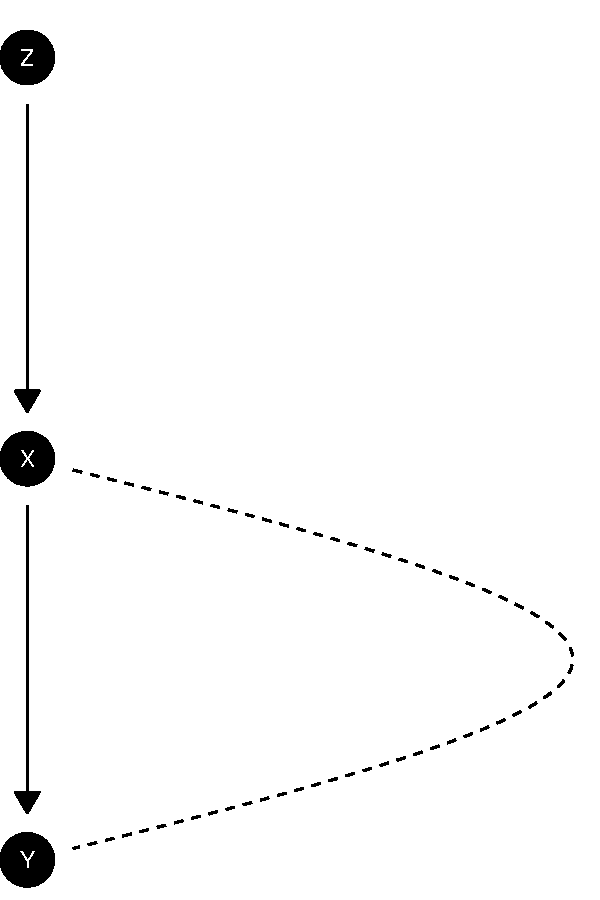
\includegraphics[width=0.5\linewidth,height=\textheight,keepaspectratio]{paper_files/figure-pdf/fig-plots-1.pdf}

}

\subcaption{\label{fig-plots-1}Without options}

\end{minipage}%
%
\begin{minipage}{0.50\linewidth}

\centering{

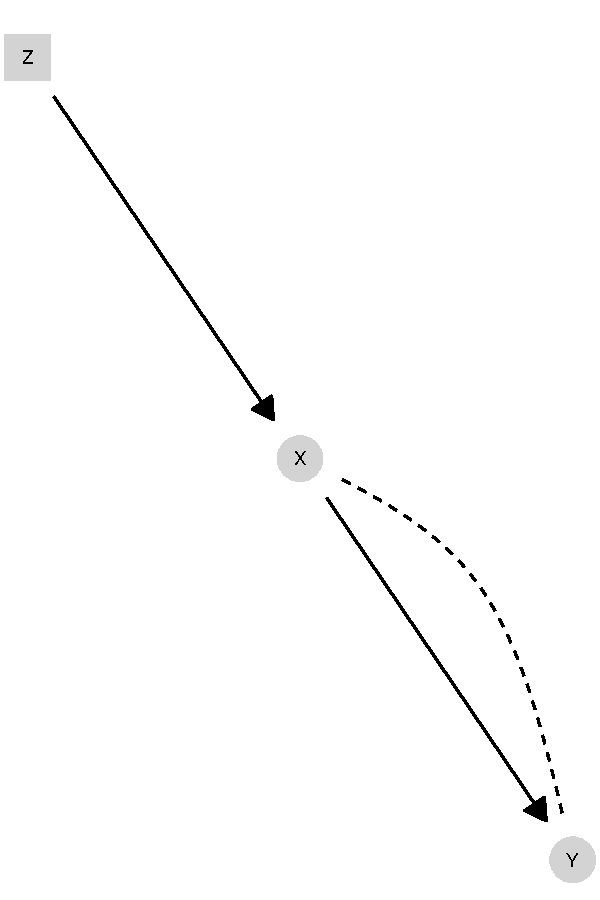
\includegraphics[width=0.5\linewidth,height=\textheight,keepaspectratio]{paper_files/figure-pdf/fig-plots-2.pdf}

}

\subcaption{\label{fig-plots-2}With options}

\end{minipage}%

\caption{\label{fig-plots}Examples of model graphs.}

\end{figure}%

\FloatBarrier

\subsection{Model inspection}\label{model-inspection}

When a model is defined, \pkg{CausalQueries} generates a set of internal
objects used for all inferential tasks. These include default parameter
values, default priors, and matrices that map parameters to causal types
and causal types to data types. Although users generally do not need to
examine these objects, \pkg{CausalQueries} provides two functions,
\texttt{inspect()} and \texttt{grab()}, that allow users to quickly
review these elements. The only difference between the two is that
\texttt{grab()} is quiet and does not produce a printout, whereas
\texttt{inspect()} does.

Table~\ref{tbl-core} summarizes features of a causal model that can be
examined using \texttt{inspect()}.

\begin{longtable}[]{@{}
  >{\raggedright\arraybackslash}p{(\linewidth - 2\tabcolsep) * \real{0.4000}}
  >{\raggedright\arraybackslash}p{(\linewidth - 2\tabcolsep) * \real{0.6000}}@{}}
\toprule\noalign{}
\begin{minipage}[b]{\linewidth}\raggedright
Element
\end{minipage} & \begin{minipage}[b]{\linewidth}\raggedright
Description
\end{minipage} \\
\midrule\noalign{}
\endfirsthead
\toprule\noalign{}
\begin{minipage}[b]{\linewidth}\raggedright
Element
\end{minipage} & \begin{minipage}[b]{\linewidth}\raggedright
Description
\end{minipage} \\
\midrule\noalign{}
\endhead
\bottomrule\noalign{}
\tabularnewline
\caption{Elements of a model that can be
inspected.}\label{tbl-core}\tabularnewline
\endlastfoot
\texttt{statement} & A character string describing causal relations
using dagitty syntax. \\
\texttt{nodes} & A list containing the nodes in the model. \\
\texttt{parents\_df} & A table listing nodes, whether they are root
nodes or not, and the number and names of parents they have. \\
\texttt{parameters} & A vector of `true' parameters. \\
\texttt{parameter\_names} & A vector of names of parameters. \\
\texttt{parameter\_mapping} & A matrix mapping from parameters into data
types. \\
\texttt{parameter\_matrix} & A matrix mapping from parameters into
causal types. \\
\texttt{parameters\_df} & A data frame containing parameter
information. \\
\texttt{causal\_types} & A data frame listing causal types and the nodal
types that produce them. \\
\texttt{nodal\_types} & A list with the nodal types of the model. \\
\texttt{data\_types} & A list with all data types consistent with the
model. \\
\texttt{ambiguities\_matrix} & A matrix mapping from causal types into
data types. \\
\texttt{prior\_hyperparameters} & A vector of alpha values used to
parameterize Dirichlet prior distributions; optionally provide node
names to reduce output. \\
\texttt{prior\_distribution} & A data frame of the parameter prior
distribution. \\
\texttt{posterior\_distribution} & A data frame of the parameter
posterior distribution. \\
\texttt{type\_prior} & A matrix of type probabilities using priors. \\
\texttt{type\_posterior} & A matrix of type probabilities using
posteriors. \\
\texttt{prior\_event\_probabilities} & A vector of data (event)
probabilities given a single realization of parameters. \\
\texttt{posterior\_event\_probabilities} & A sample of data (event)
probabilities from the posterior. \\
\texttt{data} & A data frame with data that was provided to update the
model. \\
\texttt{stan\_summary} & A \texttt{stanfit} summary with processed
parameter names. \\
\texttt{stanfit} & An unprocessed \texttt{stanfit} object as generated
by Stan. \\
\texttt{stan\_warnings} & A list of warnings produced by Stan during
updating. \\
\end{longtable}

\subsection{Tailoring models}\label{tailoring-models}

When a causal statement is provided to \texttt{make\_model()}, the model
is created with a set of default assumptions: specifically, there are no
restrictions on nodal types, and flat priors are assumed over all
parameters. These features can be modified after the model is created
using \texttt{set\_confounds}, \texttt{set\_restrictions},
\texttt{set\_priors}, and \texttt{set\_parameters}.

\subsubsection{Allowing confounding}\label{sec-confounding}

Unobserved confounding between two (or more) nodes arises when the nodal
types for the nodes are not independent. For instance, in the
\(X \rightarrow Y\) graph, there are \(2\) nodal types for \(X\) and
\(4\) for \(Y\). There are thus \(8\) joint nodal types (or causal
types), as shown in Table~\ref{tbl-joint}.

\begin{longtable}[]{@{}
  >{\centering\arraybackslash}p{(\linewidth - 6\tabcolsep) * \real{0.2500}}
  >{\centering\arraybackslash}p{(\linewidth - 6\tabcolsep) * \real{0.2500}}
  >{\centering\arraybackslash}p{(\linewidth - 6\tabcolsep) * \real{0.2500}}
  >{\centering\arraybackslash}p{(\linewidth - 6\tabcolsep) * \real{0.2500}}@{}}
\toprule\noalign{}
\begin{minipage}[b]{\linewidth}\centering
\end{minipage} & \begin{minipage}[b]{\linewidth}\centering
\(\theta^X_{0}\)
\end{minipage} & \begin{minipage}[b]{\linewidth}\centering
\(\theta^X_{1}\)
\end{minipage} & \begin{minipage}[b]{\linewidth}\centering
\(\sum\)
\end{minipage} \\
\midrule\noalign{}
\endfirsthead
\toprule\noalign{}
\begin{minipage}[b]{\linewidth}\centering
\end{minipage} & \begin{minipage}[b]{\linewidth}\centering
\(\theta^X_{0}\)
\end{minipage} & \begin{minipage}[b]{\linewidth}\centering
\(\theta^X_{1}\)
\end{minipage} & \begin{minipage}[b]{\linewidth}\centering
\(\sum\)
\end{minipage} \\
\midrule\noalign{}
\endhead
\bottomrule\noalign{}
\tabularnewline
\caption{Nodal types in an \(X \rightarrow Y\)
model.}\label{tbl-joint}\tabularnewline
\endlastfoot
\(\theta^Y_{00}\) & \(\Pr(\theta^X_0, \theta^Y_{00})\) &
\(\Pr(\theta^X_1, \theta^Y_{00})\) & \(\Pr(\theta^Y_{00})\) \\
\(\theta^Y_{10}\) & \(\Pr(\theta^X_0, \theta^Y_{10})\) &
\(\Pr(\theta^X_1, \theta^Y_{10})\) & \(\Pr(\theta^Y_{10})\) \\
\(\theta^Y_{01}\) & \(\Pr(\theta^X_0, \theta^Y_{01})\) &
\(\Pr(\theta^X_1, \theta^Y_{01})\) & \(\Pr(\theta^Y_{01})\) \\
\(\theta^Y_{11}\) & \(\Pr(\theta^X_0, \theta^Y_{11})\) &
\(\Pr(\theta^X_1, \theta^Y_{11})\) & \(\Pr(\theta^Y_{11})\) \\
\(\sum\) & \(\Pr(\theta^X_0)\) & \(\Pr(\theta^X_1)\) & 1 \\
\end{longtable}

Table~\ref{tbl-joint} has eight interior elements so that an
unconstrained joint distribution would have seven degrees of freedom. A
no-confounding assumption means that
\(\Pr(\theta^X, \theta^Y) = \Pr(\theta^X)\Pr(\theta^Y)\). In this case,
it is sufficient to put a distribution on the marginals, and there would
be \(3\) degrees of freedom for \(Y\) and \(1\) for \(X\), totaling
\(4\) rather than \(7\). To allow for an unconstrained joint
distribution, the parameters data frame for this model would include two
parameter families associated with the node \(Y\). Each family
represents the conditional distribution of \(Y\)'s nodal types, given
\(X\). For example, the parameter \texttt{Y01\_X.1} can be interpreted
as \(\Pr(\theta^Y = \theta^Y_{01} | \theta^X=1)\). Refer to
Table~\ref{tbl-lipidspar} for an example of a parameter matrix with
confounding.

The confounding structure can influence the number of parameters based
on the underlying DAG. Table~\ref{tbl-dof} demonstrates the number of
independent parameters required for different types of confounding.

\begin{longtable}{lc}

\toprule
Model & Degrees of freedom\\
\midrule
X → Y ← W & 17\\
X → Y ← W; X ←→ W & 18\\
X → Y ← W; X ←→ Y; W ←→ Y & 62\\
X → Y ← W; X ←→ Y; W ←→ Y; X ←→ W & 63\\
X → W → Y ← X & 19\\
X → W → Y ← X; W ←→ Y & 64\\
X → W → Y ← X; X ←→ W; W ←→ Y & 67\\
X → W → Y ← X; X ←→ W; W ←→ Y; X ←→ Y & 127\\
\bottomrule


\caption{\label{tbl-dof}Number of different independent parameters
(degrees of freedom) for different three-node models.}

\tabularnewline
\end{longtable}

\subsubsection{Setting restrictions}\label{restrictions}

It is often beneficial to constrain the set of types. In
\pkg{CausalQueries}, this is achieved at the nodal type level, with
restrictions on causal types following those on nodal types. For
example, in analyses of data with imperfect compliance, such as in our
Lipids model example, it is common to impose a monotonicity assumption:
that \(X\) does not decrease in response to \(Z\). This assumption is
necessary to interpret instrumental variable estimates as consistent
estimates of the complier average treatment effect. In
\pkg{CausalQueries}, we can impose this assumption by removing types for
which \(X\) decreases in \(Z\) as follows:

\begin{CodeInput}
R> model_restricted <- lipids_model |> 
+    set_restrictions("X[Z = 1] < X[Z = 0]")
\end{CodeInput}

If we wanted to retain only this nodal type rather than remove it, we
could do so by passing \texttt{keep\ =\ TRUE} as an argument to the
\texttt{set\_restrictions()} function call. Users can use
\texttt{inspect(model,\ "parameter\_matrix")} to view the resulting
parameter matrix in which both the set of parameters and the set of
causal types are restricted.

Restrictions in \pkg{CausalQueries} can be set in several other ways
described below.

\begin{itemize}
\item
  Using nodal type labels:

  \begin{CodeInput}
  R> model <- lipids_model |> set_restrictions(
  +    labels = list(X = "01", Y = c("00", "01", "11")), keep = TRUE)
  \end{CodeInput}
\item
  Using wildcards in nodal type labels:

  \begin{CodeInput}
  R> model <- lipids_model |> set_restrictions(labels = list(Y = "?0"))
  \end{CodeInput}
\item
  In models with confounding, restrictions can be added to nodal types
  conditional on the values of other nodal types using a \texttt{given}
  argument:

  \begin{CodeInput}
  R> model <- lipids_model |> set_restrictions(
  +    labels = list(Y = c('00', '11')), given = 'X.00')
  \end{CodeInput}
\end{itemize}

Setting restrictions sometimes involves using causal syntax (see
Section~\ref{sec-syntax} for a guide to the syntax used by
\pkg{CausalQueries}). The help file in \texttt{?set\_restrictions}
provides further details and examples of restrictions users can set.

\subsubsection{Setting priors}\label{priors}

Priors on model parameters can be added to the parameters data frame and
interpreted as alpha parameters of a Dirichlet distribution. The
Dirichlet distribution is a probability distribution over an \(n-1\)
dimensional unit simplex. It is a generalization of the Beta
distribution and is parameterized by an \(n\)-dimensional positive
vector \(\alpha\). For example, a Dirichlet distribution with
\(\alpha = (1, 1, 1, 1, 1)\) provides a probability distribution over
all non-negative \(5\)-dimensional vectors that sum to \(1\), such as
\((0.1, 0.1, 0.1, 0.1, 0.6)\) or \((0.1, 0.2, 0.3, 0.3, 0.1)\). This
specific value for \(\alpha\) implies that all such vectors are equally
likely. Different values for \(\alpha\) can be used to adjust the
expectation and certainty for each dimension. For instance, the vector
\(\alpha = (100, 1, 1, 1, 100)\) would place more weight on
distributions that are close to \((0.5, 0, 0, 0, 0.5)\).

In \pkg{CausalQueries}, priors are generally specified over the
distribution of nodal types.\footnote{If there is confounding in the
  model, priors are specified over the conditional distribution of nodal
  types.} For example, in a model represented by \(X \rightarrow Y\),
there is one Dirichlet distribution over the two types for \(\theta^X\)
and another Dirichlet distribution over the four types for \(\theta^Y\).
Importantly, it is implicitly assumed that priors are independent across
families. Thus, in a model represented by \(X \rightarrow Y\), we
specify beliefs over \(\lambda^X\) and \(\lambda^Y\) separately.
\pkg{CausalQueries} does not allow users to specify correlated beliefs
over these parameters.\footnote{Users can specify beliefs about
  \(\lambda^Y\) given \(\theta^X\) if a model involves possible
  confounding. However, this refers to beliefs over a joint
  distribution, not jointly distributed beliefs.}

Prior hyperparameters are set to unity by default, corresponding to
uniform priors. Users can retrieve the model's priors as follows:

\begin{CodeInput}
R> lipids_model |> inspect("prior_hyperparameters", nodes = "X") 
\end{CodeInput}

\begin{verbatim}

prior_hyperparameters
Alpha parameter values used for Dirichlet prior distributions:

X.00 X.10 X.01 X.11 
   1    1    1    1 
\end{verbatim}

Alternatively users can set Jeffreys priors using \texttt{set\_priors()}
as follows:

\begin{CodeInput}
R> model <- lipids_model |> set_priors(distribution = "jeffreys")
\end{CodeInput}

Users can also provide custom priors. The simplest way to specify custom
priors is to add them as a vector of numbers using
\texttt{set\_priors()}. For instance:

\begin{CodeInput}
R> lipids_model |> set_priors(
+    param_names = c("X.10", "X.01"), alphas = 3:4) |> 
+    inspect("prior_hyperparameters", nodes = "X")
\end{CodeInput}

\begin{verbatim}

prior_hyperparameters
Alpha parameter values used for Dirichlet prior distributions:

X.00 X.10 X.01 X.11 
   1    3    4    1 
\end{verbatim}

The priors here should be interpreted as indicating
\(\alpha_X = (1, 3, 4, 1)\), which implies a distribution over
\((\lambda^X_{00},\lambda^X_{10}, \lambda^X_{01}, \lambda^X_{11})\) with
expectation
\(\left(\frac{1}{9}, \frac{3}{9}, \frac{4}{9}, \frac{1}{9} \right)\).

Providing priors as a vector of numbers for larger models can be hard.
For that reason, \texttt{set\_priors()} allows for more targeted
modifications of the parameter vector. For instance:

\begin{CodeInput}
R> lipids_model |> set_priors(
+    statement = "X[Z = 1] > X[Z = 0]", alphas = 3) |>
+    inspect("prior_hyperparameters", nodes = "X")
\end{CodeInput}

\begin{verbatim}

prior_hyperparameters
Alpha parameter values used for Dirichlet prior distributions:

X.00 X.10 X.01 X.11 
   1    1    3    1 
\end{verbatim}

While setting highly targeted priors is convenient and flexible, it
should be done with caution. Assigning priors to specific parameters in
complex models, particularly those involving confounding, can
significantly impact inferences (see \citet{richardson2011transparent}
on an approach to specifying priors that more clearly separates beliefs
over identifies and non-identified components). Additionally, note that
flat priors over nodal types do not necessarily equate to flat priors
over queries. Flat priors over parameters within a parameter family
assign equal weight to each nodal type, which can lead to strong
assumptions about causal quantities of interest. For example, in an
\(X \rightarrow Y\) model where negative effects are excluded, the
average causal effect implied by flat priors is \(1/3\). This can be
demonstrated by querying the model as follows:

\begin{CodeInput}
R> query <- make_model("X -> Y") |> 
+    set_restrictions(decreasing("X", "Y")) |>
+    query_model("Y[X = 1] - Y[X = 0]", using = "priors")
\end{CodeInput}

More subtly, the \emph{structure} of a model, coupled with flat priors,
has substantive importance for priors on causal quantities. For
instance, with flat priors, prior on the probability that \(X\) has a
positive effect on \(Y\) in the model \(X \rightarrow Y\) is centered on
\(1/4\). But prior on the probability that \(X\) positively affects
\(Y\) in the model \(X \rightarrow M \rightarrow Y\) is centered on
\(1/8\). Caution regarding priors is essential when queries are not
identified, as is the case for many models considered here. For some
quantities, the marginal posterior distribution reflects the marginal
prior distribution \citep{poirier_revising_1998}.

\subsubsection{Setting parameters}\label{parameters}

By default, models include a vector of parameter values within the
\texttt{parameters\_df} data frame. These values are useful for
generating data or for scenarios like process tracing, where inferences
about causal types (\(\theta\)) are made from case-level data, assuming
the model is known. The process of setting parameters is similar to
setting priors. The key difference is that while the \(\alpha\) value
assigned to nodal types can be any positive number---reflecting our
confidence in the parameter value---the parameter values themselves must
be within the unit interval, \([0,1]\). If parameter values provided are
outside this interval, they are normalized to fit within it.

The causal model below has two parameter sets, one for \(X\) and one for
\(Y\), with two nodal types for \(X\) and four for \(Y\). The key
feature of the parameters is that they must sum to \(1\) within each
parameter set.

\begin{CodeInput}
R> make_model("X -> Y") |> inspect("parameters")
\end{CodeInput}

\begin{verbatim}

parameters
Model parameters with associated probabilities: 

 X.0  X.1 Y.00 Y.10 Y.01 Y.11 
0.50 0.50 0.25 0.25 0.25 0.25 
\end{verbatim}

The example below illustrates a change in the value of the parameter
that corresponds to a positive effect of \(X\) on \(Y\). Here, the nodal
type \texttt{Y.Y01} is set to be \(0.7\), while the other nodal types of
this parameter set were re-normalized so that the parameters in the set
still sum up to one.

\begin{CodeInput}
R> make_model("X -> Y") |> set_parameters(
+    statement = "Y[X = 1] > Y[X = 0]", parameters = .7) |>
+    inspect("parameters")
\end{CodeInput}

\begin{verbatim}

parameters
Model parameters with associated probabilities: 

 X.0  X.1 Y.00 Y.10 Y.01 Y.11 
 0.5  0.5  0.1  0.1  0.7  0.1 
\end{verbatim}

\subsection{Drawing and manipulating
data}\label{drawing-and-manipulating-data}

Once a model has been defined, it is possible to simulate data from the
model using the \texttt{make\_data()} function. For instance, this can
be useful for assessing a model's expected performance given data drawn
from some speculated set of parameter values.

\subsubsection{Drawing data basics}\label{drawing-data-basics}

Generating data requires a specification of parameter values. The
parameter values in the parameters data frame are used by default.
Otherwise users can provide parameters on the fly.

\begin{CodeInput}
R> lipids_model |> make_data(n = 4)
\end{CodeInput}

\begin{verbatim}
  Z X Y
1 0 1 1
2 1 0 0
3 1 1 1
4 1 1 1
\end{verbatim}

The resulting data is ordered by data type, as shown in the example
above. Users can also specify parameters directly or draw parameters
from a prior or posterior distribution by specifying
\texttt{param\_type} argument in the \texttt{make\_data()} call.

\subsubsection{Drawing incomplete data}\label{drawing-incomplete-data}

\pkg{CausalQueries} can be used when researchers have gathered different
amounts of data for different nodes. For example, a researcher might
gather data on \(X\) and \(Y\) for all units, but only have data on
\(M\) for some units. The \texttt{make\_data()} function enables users
to simulate such data by specifying a data strategy that outlines the
probabilities of observing data for different nodes, potentially based
on previously observed nodes.

\begin{CodeInput}
R> sample_data <- lipids_model |> make_data(
+    n = 8, nodes = list(c("Z", "Y"), "X"), probs = list(1, .5),
+    subsets = list(TRUE, "Z == 1 & Y == 0"))
\end{CodeInput}

\subsubsection{Reshaping data}\label{reshaping-data}

Data produced by \texttt{make\_data()} typically comes in a ``long''
format, where each row represents a single observation. However, it can
be useful to have data a ``compact'' format that summarizes the number
of units for each data type, organized by data ``strategy,'' indicating
the nodes for which data was collected. The \pkg{CausalQueries} package
provides function \texttt{collapse\_data()} that allow users to convert
data to compact format.

\begin{CodeInput}
R> sample_data |> collapse_data(lipids_model)
\end{CodeInput}

\begin{verbatim}
    event strategy count
1  Z0X0Y0      ZXY     0
2  Z1X0Y0      ZXY     0
3  Z0X1Y0      ZXY     0
4  Z1X1Y0      ZXY     0
5  Z0X0Y1      ZXY     1
6  Z1X0Y1      ZXY     0
7  Z0X1Y1      ZXY     0
8  Z1X1Y1      ZXY     0
9    Z0Y0       ZY     2
10   Z1Y0       ZY     1
11   Z0Y1       ZY     2
12   Z1Y1       ZY     2
\end{verbatim}

In the same way, it is possible to move from compact to long format
using \texttt{expand\_data()}.\footnote{Note that \texttt{NA}'s are
  interpreted as data not being sought.}

\section{Updating models}\label{sec-update}

The approach used by the \pkg{CausalQueries} package to update parameter
values given observed data relies on the Stan programming language
\citep{carpenter_stan_2017}. Below we explain the data required by the
generic Stan program implemented in the package, the structure of that
program, and then show how to use the package to produce posterior draws
of parameters.

\subsection{Data for Stan}\label{data-for-stan}

We use a generic Stan program that works for all binary causal models.
The main advantage of the generic program is that it allows us to pass
the details of the causal model as data inputs to Stan instead of
generating individual Stan programs for each causal model.
\hyperref[sec-stancode]{Appendix B} provides the complete Stan model
code.

The data required by the Stan program includes vectors of observed data
and priors on parameters, as well as a set of matrices needed for the
mapping between events, data types, causal types, and parameters. In
addition, data passed to \texttt{stan} includes counts of all relevant
quantities as well as start and end positions of parameters pertaining
to specific nodes and distinct data strategies. The internal function
\texttt{prep\_stan\_data()} takes the model and data as arguments and
produces a list with all objects that are required by the generic Stan
program. Package users do not need to call the
\texttt{prep\_stan\_data()} function directly.

\subsection{How the Stan program
works}\label{how-the-stan-program-works}

The Stan model involves the following elements: (1) a specification of
priors over sets of parameters, (2) a mapping from parameters to event
probabilities, and (3) a likelihood function. Below, we describe each of
those elements in more detail.

\subsubsection{Probability distributions over parameter
sets}\label{probability-distributions-over-parameter-sets}

The causal structure provided by a DAG simplifies the problem of
generating a probability distribution over all parameters by focusing on
distributions over sets of parameters. In the absence of unobserved
confounding, these sets correspond to the nodal types for each node,
resulting in a probability distribution over these nodal types. For
example, in the \(X \rightarrow Y\) model, there are two parameter sets.
The \(X\) nodal types are represented by a 2-dimensional Dirichlet
distribution,
\((\lambda^X_0, \lambda^X_1) \sim \text{Dirichlet}(\alpha^X_0, \alpha^X_1)\),
and the \(Y\) nodal types are represented by a \(4\)-dimensional
Dirichlet distribution,
\((\lambda^Y_{00}, \lambda^Y_{10}, \lambda^Y_{01}, \lambda^Y_{11}) \sim \text{Dirichlet}(\alpha^Y_{00}, \alpha^Y_{10}, \alpha^Y_{01}, \alpha^Y_{11})\).

In cases involving confounding, these parameter sets are defined for a
given node, conditional on the values of other nodes.

\subsubsection{Event probabilities}\label{event-probabilities}

We calculate the probability of data types for any parameter vector
\(\lambda\). This is done using a matrix that maps from parameters into
data types.

In cases without confounding, there is a column for each data type; the
matrix indicates which nodes in each set ``contribute'' to the data
type, and the probability of the data type is found by summing within
sets and taking the product over sets. To illustrate, we can examine the
parameter mapping matrix for a simple model using the \texttt{inspect()}
function as follows:

\begin{CodeInput}
R> make_model("X -> Y") |> inspect("parameter_mapping") 
\end{CodeInput}

\begin{verbatim}

parameter_mapping (Parameter mapping matrix) 

  Maps from parameters to data types, with
  possibly multiple columns for each data type
  in cases with confounding. 

     X0Y0 X1Y0 X0Y1 X1Y1
X.0     1    0    1    0
X.1     0    1    0    1
Y.00    1    1    0    0
Y.10    0    1    1    0
Y.01    1    0    0    1
Y.11    0    0    1    1
\end{verbatim}

The probability of each data type can be determined using the parameter
mapping matrix by combining a parameter vector with the corresponding
column of the matrix. For instance, in the model above, the probability
of the data type \texttt{X0Y0}, denoted as \(w_{00}\), is calculated as
\(\lambda^X_0 \times (\lambda^Y_{00} + \lambda^Y_{01})\). This
represents the product of the probability of \texttt{X.0} and the sum of
the probabilities for \texttt{Y.00} and \texttt{Y.01}.

In cases with confounding, the approach is similar, except that the
parameter mapping matrix can contain multiple columns for each data type
to capture non-independence between nodes.

In the case of incomplete data, we first identify the set of data
strategies, where a collection of a data strategy might be of the form
``gather data on \(X\) and \(M\), but not \(Y\), for \(n_1\) cases and
gather data on \(X\) and \(Y\), but not \(M\), for \(n_2\) cases.''
Within a data strategy, the probability of an observed event is given by
summing the probabilities of the types that could give rise to a
particular pattern of incomplete data.

\subsubsection{Data probability}\label{data-probability}

Once we have the event probabilities in hand for each data strategy, we
are ready to calculate the probability of the data. For a given data
strategy, this is given by a multinomial distribution with these event
probabilities. When there is incomplete data, and so there are multiple
data strategies, the probability of the data is given by the product of
the multinomial probabilities for data generated by each strategy.

\subsection{Implementation}\label{implementation}

The \texttt{update\_model()} function is used to update a model by
appending a posterior distribution over the model parameters. This
function utilizes \texttt{rstan::sampling()} to draw from the posterior
distribution, and users can pass any additional arguments that
\texttt{rstan::sampling()} accepts. Since model updating can be slow for
complex models, \hyperref[sec-parallel]{Appendix A} demonstrates how
users can employ parallelization to enhance computation speed.
\hyperref[sec-benchmark]{Appendix C} offers an overview of model
updating benchmarks, assessing the impact of model complexity and data
size on updating times.

Users have the option to provide a \texttt{data} argument when calling
\texttt{update\_model()}. This argument should be a data frame that
includes some or all of the nodes in the model. It is optional; if no
data is provided, the Stan model will still run, and the resulting
posterior distribution added to the model will be interpreted as draws
from the prior distribution.

\subsection{Incomplete and censored
data}\label{incomplete-and-censored-data}

\pkg{CausalQueries} assumes that missing data is missing at random,
conditional on observed data. For instance, in an
\(X \rightarrow M \rightarrow Y\) model, a researcher might have chosen
to collect data on \(M\) in a random set of cases in which \(X=1\) and
\(Y=1\). If there are positive relations at each stage, one may be more
likely to observe \(M\) in cases in which \(M=1\). However, the
observation of \(M\) is still random and conditional on the observed
\(X\) and \(Y\) data. The Stan model in \pkg{CausalQueries} takes
account of this kind of sampling by assessing the probability of
observing a particular pattern of data within each data
strategy.\footnote{For further discussion, see Section 9.2.3.2 in
  \citet{humphreys_integrated_2023}.}

Additionally, you can specify when data has been censored, allowing the
Stan model to account for it. For example, consider a scenario where we
only observe \(X\) when \(X=1\) and not when \(X=0\). This type of
sampling is non-random and depends on observable variables. You can
address this by informing Stan that the probability of observing a
particular data type is \(0\), regardless of parameter values. This is
achieved using the \texttt{censored\_types} argument in
\texttt{update\_model()}.

To illustrate, in the example below, we observe perfectly correlated
data for \(X\) and \(Y\). If we are aware that data in which
\(X \neq Y\) has been censored, then when we update, we do not move
towards a belief that \(X\) causes \(Y\).

\begin{CodeInput}
R> data <- data.frame(X = rep(0:1, 5), Y = rep(0:1, 5))
R> list(uncensored = update_model(make_model("X -> Y"), 
+    data = data, refresh = 0),
+    censored = update_model(make_model("X -> Y"), data = data, 
+    censored_types = c("X1Y0",  "X0Y1"), refresh = 0)) |>
+    query_model("Y[X = 1] - Y[X = 0]", using = "posteriors") |>
+    dplyr::select(-using)
\end{CodeInput}

\begin{verbatim}

Causal queries generated by query_model

|model      |case_level |  mean|    sd| cred.low| cred.high|
|:----------|:----------|-----:|-----:|--------:|---------:|
|uncensored |FALSE      | 0.590| 0.196|    0.145|     0.897|
|censored   |FALSE      | 0.015| 0.318|   -0.625|     0.641|
\end{verbatim}

\subsection{Output}\label{output}

The main output of the \texttt{update\_model()} function is a model that
includes a posterior distribution of the model parameters, stored as a
data frame within the model list. You can access this posterior
distribution directly using the \texttt{grab()} function (or use the
\texttt{inspect()} function for a more detailed output) as shown below:

\begin{CodeInput}
R> model <- make_model("X -> Y") |> update_model()
R> posterior <- inspect(model, "posterior_distribution")  
\end{CodeInput}

Additionally, a distribution of causal types is stored by default.
Optionally, the \texttt{stanfit} object and a distribution over event
probabilities can also be saved as shown below:

\begin{CodeInput}
R> lipids_model <- lipids_model |> update_model(
+    keep_fit = TRUE, keep_event_probabilities = TRUE)
\end{CodeInput}

The summary of the Stan model can be accessed using \texttt{inspect()}
function and is saved in the updated model object by default.

\begin{CodeInput}
R> make_model("X -> Y") |> update_model(keep_type_distribution = FALSE, 
+    refresh = 0) |> inspect("stan_summary") 
\end{CodeInput}

\begin{verbatim}

stan_summary
Stan model summary:

Inference for Stan model: simplexes.
4 chains, each with iter=2000; warmup=1000; thin=1; 
post-warmup draws per chain=1000, total post-warmup draws=4000.

                   mean se_mean   sd   2.5%   25%   50%   75% 97.5% n_eff Rhat
X.0                0.49    0.01 0.29   0.02  0.24  0.49  0.75  0.97  2976 1.00
X.1                0.51    0.01 0.29   0.03  0.25  0.51  0.76  0.98  2976 1.00
Y.00               0.25    0.01 0.19   0.01  0.09  0.20  0.37  0.71  1419 1.00
Y.10               0.25    0.00 0.19   0.01  0.09  0.20  0.37  0.71  4026 1.00
Y.01               0.25    0.00 0.19   0.01  0.09  0.21  0.37  0.71  4142 1.00
Y.11               0.25    0.00 0.20   0.01  0.09  0.20  0.37  0.71  4265 1.00
lp__               1.02    0.02 1.00   0.03  0.29  0.71  1.43  3.75  2419 1.00
log_sum_gammas[2]  1.86    0.05 1.27   0.34  0.99  1.59  2.42  4.99   649 1.01
lp__              -7.58    0.05 1.72 -11.74 -8.44 -7.17 -6.34 -5.43  1185 1.00

Samples were drawn using NUTS(diag_e) at Wed Jul 30 16:19:14 2025.
For each parameter, n_eff is a crude measure of effective sample size,
and Rhat is the potential scale reduction factor on split chains (at 
convergence, Rhat=1).
\end{verbatim}

This summary provides information on the distribution of parameters and
convergence diagnostics, summarized in the \texttt{Rhat} column. The
last row shows the unnormalized log density on Stan's unconstrained
space, which is intended to diagnose sampling efficiency and evaluate
approximations.\footnote{See
  \href{https://mc-stan.org/cmdstanr/reference/fit-method-lp.html}{Stan
  documentation} for more details.} This summary can also include
summaries for the transformed parameters if users retain these.

\subsection{Convergence problems and
diagnostics}\label{convergence-problems-and-diagnostics}

There is no guarantee that updating will produce reliable posterior
draws. Indeed for some models, convergence failure are predictable.
Fortunately, \texttt{stan} provides warnings that alert users to
possible problems. These warnings are retained by \pkg{CausalQueries}
and repeated in model summaries or when queries are posed.

In the example below the missing data on \(M\) means that there is no
information to assess whether the strong relation between \(X\) and
\(Y\) is due to positive effects.

\begin{CodeInput}
R> model <- make_model("X -> M -> Y") |> update_model(
+    data = data.frame(X = rep(0:1, 10000), Y = rep(0:1, 10000)), 
+    iter = 5000, refresh = 0)
\end{CodeInput}

The print and summary methods returns warnings alerting users to the
problem thus:

\begin{CodeInput}
R> model
\end{CodeInput}

\begin{verbatim}

Causal statement: 
M -> Y; X -> M

Number of nodal types by node:
X M Y 
2 4 4 

Number of causal types: 32

Model has been updated and contains a posterior distribution with
4 chains, each with iter=5000; warmup=2500; thin=1;  
Use inspect(model, 'stan_summary') to inspect stan summary

Warnings passed from rstan during updating:
The largest R-hat is 1.53, indicating chains have not mixed
Bulk Effective Samples Size (ESS) is too low
Tail Effective Samples Size (ESS) is too low 
\end{verbatim}

If users wish to run more advanced diagnostics of performance, they can
retain and access the ``raw'' Stan output as follows:

\begin{CodeInput}
R> model <- make_model("X -> Y") |> 
+    update_model(refresh = 0, keep_fit = TRUE)
\end{CodeInput}

Note that the raw output uses labels from the generic Stan model:
\texttt{lambda} for the vector of parameters, corresponding to the
parameters in the parameters data frame
(\texttt{inspect(model,\ "parameters\_df")}), a vector \texttt{types}
for the causal types (\texttt{inspect(model,\ "causal\_types")}) and
\texttt{event\_probabilities} for the event probabilities
(\texttt{inspect(model,\ "event\_probabilities")}).

\begin{CodeInput}
R> model |> inspect("stanfit")
\end{CodeInput}

\begin{verbatim}

stanfit
Stan model summary:
Inference for Stan model: simplexes.
4 chains, each with iter=2000; warmup=1000; thin=1; 
post-warmup draws per chain=1000, total post-warmup draws=4000.

                   mean se_mean   sd   2.5%   25%   50%   75% 97.5% n_eff Rhat
lambdas[1]         0.50    0.01 0.29   0.03  0.25  0.49  0.74  0.97  3036 1.00
lambdas[2]         0.50    0.01 0.29   0.03  0.26  0.51  0.75  0.97  3036 1.00
lambdas[3]         0.25    0.00 0.19   0.01  0.09  0.21  0.37  0.70  2031 1.00
lambdas[4]         0.25    0.00 0.19   0.01  0.09  0.21  0.37  0.71  4633 1.00
lambdas[5]         0.25    0.00 0.20   0.01  0.09  0.20  0.37  0.72  4162 1.00
lambdas[6]         0.25    0.00 0.20   0.01  0.09  0.20  0.37  0.71  4701 1.00
log_sum_gammas[1]  1.00    0.02 0.96   0.03  0.30  0.72  1.39  3.43  2536 1.00
log_sum_gammas[2]  1.85    0.03 1.19   0.36  1.00  1.58  2.41  4.93  1159 1.01
types[1]           0.12    0.00 0.13   0.00  0.03  0.08  0.18  0.50  2065 1.00
types[2]           0.13    0.00 0.13   0.00  0.03  0.08  0.18  0.48  2390 1.00
types[3]           0.12    0.00 0.13   0.00  0.03  0.08  0.18  0.50  3785 1.00
types[4]           0.13    0.00 0.13   0.00  0.03  0.08  0.18  0.49  3407 1.00
types[5]           0.12    0.00 0.13   0.00  0.03  0.08  0.18  0.48  3507 1.00
types[6]           0.13    0.00 0.13   0.00  0.03  0.08  0.18  0.49  3619 1.00
types[7]           0.12    0.00 0.13   0.00  0.03  0.08  0.17  0.49  3841 1.00
types[8]           0.13    0.00 0.13   0.00  0.03  0.08  0.19  0.49  3863 1.00
lp__              -7.53    0.04 1.65 -11.75 -8.37 -7.15 -6.32 -5.44  1368 1.00

Samples were drawn using NUTS(diag_e) at Wed Jul 30 16:19:16 2025.
For each parameter, n_eff is a crude measure of effective sample size,
and Rhat is the potential scale reduction factor on split chains (at 
convergence, Rhat=1).
\end{verbatim}

Users can then pass the \texttt{stanfit} object to other diagnostic
packages such as \pkg{bayesplot}.

\section{Queries}\label{sec-query}

\pkg{CausalQueries} provides functionality to pose and answer elaborate
causal queries. The key approach is to code causal queries as functions
of causal types and return a distribution over the queries implied by
the distribution over causal types. The primary approach is to use
\texttt{query\_model()} to generate an object of class
\texttt{model\_query} (see Section~\ref{sec-classes}) which prints to a
table or can be plotted directly. The next sections describe how such
queries are calculated and the syntax used for posing queries.

\subsection{Calculating factual and counterfactual
quantities}\label{sec-propagation}

An essential step in calculating most queries is assessing what outcomes
will arise for causal types given different interventions on nodes. In
practice, we map from causal types to data types by propagating realized
values on nodes forward in the DAG, moving from exogenous or intervened
upon nodes to their descendants in generational order. An internal
function, \texttt{realise\_outcomes()}, achieves this by traversing the
DAG while recording the values implied by realizations on the node's
parents for each node's nodal types.

To illustrate, consider the first causal type of a \(X \rightarrow Y\)
model:

\begin{enumerate}
\def\labelenumi{\arabic{enumi}.}
\tightlist
\item
  \(\theta^X_0\) implies that, absent intervention on \(X\), \(X\) has a
  realized value of \(0\); \(\theta^Y_{00}\) implies that, absent
  intervention on \(Y\), \(Y\) has a realized value of \(0\) regardless
  of \(X\).
\item
  We substitute for \(Y\) the value implied by the \(00\) nodal type
  given a \(0\) value on \(X\), which in turn is \(0\).
\end{enumerate}

The \texttt{realise\_outcomes()} function, when called on this model,
outputs the realized values for all causal types, with row names
indicating the corresponding causal types.

\begin{CodeInput}
R> make_model("X -> Y") |> realise_outcomes()
\end{CodeInput}

\begin{verbatim}
     X Y
0.00 0 0
1.00 1 0
0.10 0 1
1.10 1 0
0.01 0 0
1.01 1 1
0.11 0 1
1.11 1 1
\end{verbatim}

Intervening on \(X\) \citep[see][]{pearl_causality_2009} with
\(do(X=1)\) yields:

\begin{CodeInput}
R> make_model("X -> Y") |> realise_outcomes(dos = list(X = 1))
\end{CodeInput}

\begin{verbatim}
     X Y
0.00 1 0
1.00 1 0
0.10 1 0
1.10 1 0
0.01 1 1
1.01 1 1
0.11 1 1
1.11 1 1
\end{verbatim}

Similarly, \texttt{realise\_outcomes()} can return the realized values
on all nodes for each causal type given arbitrary interventions.

\subsection{Causal syntax}\label{sec-syntax}

\pkg{CausalQueries} provides syntax for the formulation of various
causal queries including queries on all rungs of the ``causal ladder''
\citep{pearl_causality_2009}: prediction, such as the proportion of
units where \(Y\) equals \(1\); intervention, such as the probability
that \(Y = 1\) when \(X\) is \emph{set} to \(1\); counterfactuals, such
as the probability that \(Y\) would be \(1\) were \(X = 1\) given we
know \(Y\) is \(0\) when \(X\) was observed to be \(0\). Queries can be
posed at the population level or case level and can be unconditional
(e.g., what is the effect of \(X\) on \(Y\) for all units) or
conditional (for example, the effect of \(X\) on \(Y\) for units for
which \(Z\) affects \(X\)). This syntax enables users to write arbitrary
causal queries to interrogate their models.

The core of querying involves determining which causal types correspond
to specific queries. Users can use logical statements to inquire about
observed conditions without interventions for factual queries. For
instance, consider the query about the proportion of units where \(Y\)
equals \(1\), expressed as \texttt{"Y\ ==\ 1"}. Here, the logical
operator \texttt{==} signifies that \pkg{CausalQueries} should consider
units that meet the strict equality condition where \(Y\) equals
\(1\).\footnote{\pkg{CausalQueries} also accepts \texttt{=} as a
  shorthand for \texttt{==}, but \texttt{==} is preferred as it is the
  standard logical operator.} When this query is executed, the
\texttt{get\_query\_types()} function identifies all types that result
in \(Y=1\) without any interventions.

\begin{CodeInput}
R> make_model("X -> Y")  |> get_query_types("Y == 1")
\end{CodeInput}

\begin{verbatim}

Causal types satisfying query's condition(s)  

 query =  Y==1 

X0.Y10  X1.Y01
X0.Y11  X1.Y11


 Number of causal types that meet condition(s) =  4
 Total number of causal types in model =  8
\end{verbatim}

The key to forming causal queries is being able to ask about the values
of variables, given that the values of some other variables are
``controlled.'' This corresponds to the application of the \(do\)
operator in \citet{pearl_causality_2009}. In \pkg{CausalQueries}, this
is done by putting square brackets, \texttt{{[}\ {]}}, around variables
that are intervened upon.

For instance, consider the query \texttt{Y{[}X\ =\ 0{]}\ ==\ 1}. This
query asks about the types for which \(Y\) equals \(1\) when \(X\) is
set to \(0\). Since \(X\) is set to zero, \(X\) is placed inside the
brackets. Given that \(Y\) equals \(1\) is a condition about potentially
observed values, it is expressed using the logical operator \texttt{==}.
The set of causal types that meets this query is quite different:

\begin{CodeInput}
R> make_model("X -> Y") |> get_query_types("Y[X = 0] == 1")
\end{CodeInput}

\begin{verbatim}

Causal types satisfying query's condition(s)  

 query =  Y[X=0]==1 

X0.Y10  X1.Y10
X0.Y11  X1.Y11


 Number of causal types that meet condition(s) =  4
 Total number of causal types in model =  8
\end{verbatim}

When a node has multiple parents, it is possible to set the values of
none, some, or all of the parents. For instance if \(X1\) and \(X2\) are
parents of \(Y\) then \texttt{Y\ ==\ 1},
\texttt{Y{[}X1\ =\ 1{]}\ ==\ 1}, and
\texttt{Y{[}X1\ =\ 1,\ X2\ =\ 1{]}\ ==\ 1} queries cases for which
\(Y=1\) when, respectively, neither parents values are controlled, when
\(X1\) is set to \(1\) but \(X2\) is not controlled, and when both
\(X1\) and \(X2\) are set to \(1\). For instance:

\begin{CodeInput}
R> make_model("X1 -> Y <- X2")  |> get_query_types(
+    "X1 == 1 & X2 == 1 & (Y[X1 = 1, X2 = 1] > Y[X1 = 0, X2 = 0])")
\end{CodeInput}

\begin{verbatim}

Causal types satisfying query's condition(s)  

 query =  X1==1&X2==1&(Y[X1=1,X2=1]>Y[X1=0,X2=0]) 

X11.X21.Y0001  X11.X21.Y0101
X11.X21.Y0011  X11.X21.Y0111


 Number of causal types that meet condition(s) =  4
 Total number of causal types in model =  64
\end{verbatim}

In this case, the aim is to identify the types for which in fact
\(X1=1\) and \(X2=1\) and, \emph{in addition}, \(Y=0\) when
\(X1 = X2 = 0\) and \(Y = 1\) when \(X1 = X2 = 1\).

\subsubsection{Conditional queries}\label{conditional-queries}

Many queries of interest are ``conditional'' queries. For example, the
effect of \(X\) on \(Y\) for units for which \(W=1\) or the effect of
\(X\) on \(Y\) for units for which \(Z\) positively affects \(X\). Such
conditional queries are posed in \pkg{CausalQueries} by providing a
\texttt{given} statement and the \texttt{query} statement or by placing
the condition following a \texttt{:\textbar{}:} separator in the query
expression. For instance
\texttt{"Y{[}X\ =\ 1{]}\ ==\ 1\ :\textbar{}:\ X\ ==\ 0"} asks for the
probability that \(Y=1\) when \(X\) is set to 1 for a case in which in
fact \(X=0\). The entire query then becomes: for what units does the
\texttt{query} condition hold among those units for which the
\texttt{given} condition holds? The two parts can each be calculated
using \texttt{get\_query\_types}. Thus, for instance, in an
\(X \rightarrow Y\) model, the probability that \(X\) causes \(Y\) given
\(X=1 \, \& \, Y=1\) is the probability of causal \texttt{X1.Y11} type
divided by the sum of the probabilities of types \texttt{X1.Y11} and
\texttt{X1.Y01}. In practice, this is done automatically for users when
they call \texttt{query\_model()} or \texttt{query\_distribution()}.

\subsubsection{Complex expressions}\label{complex-expressions}

Many queries involve complex statements across multiple sets of types,
which can be constructed using relational operators. For instance, users
can query whether \(X\) has a positive effect on \(Y\) by checking if
\(Y\) is greater when \(X\) is set to \(1\) compared to when \(X\) is
set to \(0\). This is expressed as
\texttt{"Y{[}X\ =\ 1{]}\ \textgreater{}\ Y{[}X\ =\ 0{]}"}. The query
``\(X\) has some effect on \(Y\)'' is given by
\texttt{"Y{[}X\ =\ 1{]}\ !=\ Y{[}X\ =\ 0{]}"}.

Linear operators can also be used over a set of simple statements. Thus
\texttt{"Y{[}X\ =\ 1{]}\ -\ Y{[}X\ =\ 0{]}"} returns the average
treatment effect. In essence, rather than returning a \texttt{TRUE} or
\texttt{FALSE} for the two parts of the query, the case memberships are
forced to numeric values (\(1\) or \(0\)), and the differences are
taken, which can be a \(1\), \(0\) or \(-1\) depending on the causal
type. Averaging provides the share of cases with positive effects, less
the share of cases with negative effects.

\begin{CodeInput}
R> make_model("X -> Y") |> get_query_types("Y[X = 1] - Y[X = 0]")
\end{CodeInput}

\begin{verbatim}
X0.Y00 X1.Y00 X0.Y10 X1.Y10 X0.Y01 X1.Y01 X0.Y11 X1.Y11 
     0      0     -1     -1      1      1      0      0 
\end{verbatim}

\subsubsection{Nested queries}\label{nested-queries}

\pkg{CausalQueries} lets users pose nested ``complex counterfactual''
queries. Rather than stipulating a value to which some node is to be
set, the user can set the value to the value that the node would take
given actions taken on ancestor nodes. For instance
\texttt{"Y{[}M\ =\ M{[}X\ =\ 0{]},\ X\ =\ 1{]}\ ==\ 1"} queries the
types for which \(Y\) equals \(1\) when \(X\) is set to \(1\), while
keeping \(M\) constant at whatever value it would take if \(X\) were set
to \(0\). Such values are important for defining queries such as the
``natural direct effect'' \citep{pearl2022direct}.

\subsection{Quantifying queries}\label{quantifying-queries}

To provide a \emph{quantitative} answer to a query, it is necessary to
assign probabilities to the causal types that correspond to the query.

\subsubsection{Queries by hand}\label{queries-by-hand}

Queries can be calculated directly from the prior distribution or the
posterior distribution provided by Stan. For instance, the following
call plots the posterior distribution for the probability that \(Y\) is
increasing in \(X\) for the \(X \rightarrow Y\) model. The resulting
plot is shown in Figure~\ref{fig-posterior-dist}.

\begin{CodeInput}
R> data  <- data.frame(X = rep(0:1, 50), Y = rep(0:1, 50))
R> model <-  make_model("X -> Y") |> update_model(
+    data, iter = 4000, refresh = 0)
R> model |> grab("posterior_distribution")  |> 
+    ggplot(aes(Y.01 - Y.10)) + geom_histogram() 
\end{CodeInput}

\begin{figure}[t]

\centering{

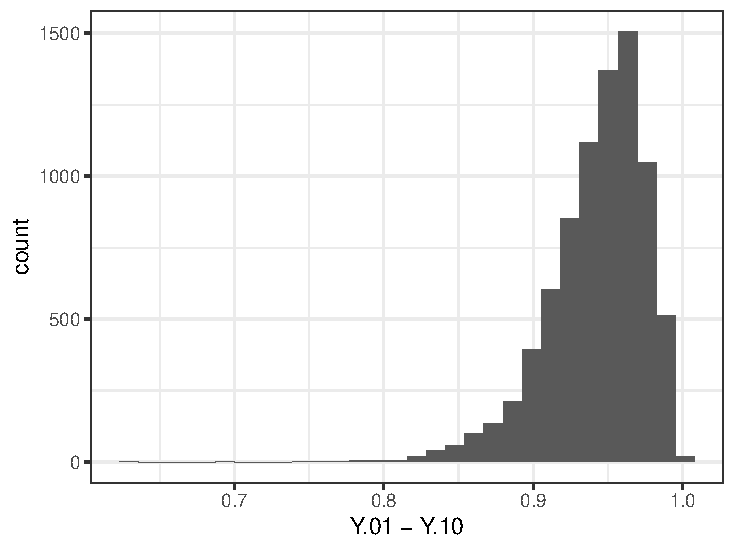
\includegraphics[width=0.6\linewidth,height=\textheight,keepaspectratio]{paper_files/figure-pdf/fig-posterior-dist-1.pdf}

}

\caption{\label{fig-posterior-dist}Posterior on ``Probability \(Y\) is
increasing in \(X\)''.}

\end{figure}%

\FloatBarrier

\subsubsection{Query distribution}\label{query-distribution}

It is generally helpful to use causal syntax to define the query and
calculate the query with respect to the prior or posterior probability
distributions. This can be done for a list of queries using
\texttt{query\_distribution()} function as follows:

\begin{CodeInput}
R> queries <- make_model("X -> Y") |> query_distribution(
+    query = list(increasing = "(Y[X = 1] > Y[X = 0])", 
+    ATE = "(Y[X = 1] - Y[X = 0])"), using = "priors")
\end{CodeInput}

The result is a data frame with one column per query and rows for draws
from prior or posterior distributions as requested.

The core function \texttt{query\_model} implements
\texttt{query\_distribution} and reports summaries of distributions.

\subsubsection{Case queries}\label{case-queries}

The commands \texttt{query\_distribution()} and \texttt{query\_model()}
can also be used when one is interested in assessing the value of a
query about a new case that we might confront.

In a sense, this is equivalent to posing a conditional query, querying
conditional on values in a case. For instance, we might consult our
posterior for the Lipids model and ask about the effect of \(X\) on
\(Y\) for a case in which \(Z=1\), \(X=1\) and \(Y=1\).

\begin{CodeInput}
R> lipids_model |> query_model(
+    query = "Y[X = 1] - Y[X = 0] :|: X == 1 & Y == 1 & Z == 1",
+    using = "posteriors") |> plot()
\end{CodeInput}

\begin{figure}[H]

\centering{

\pandocbounded{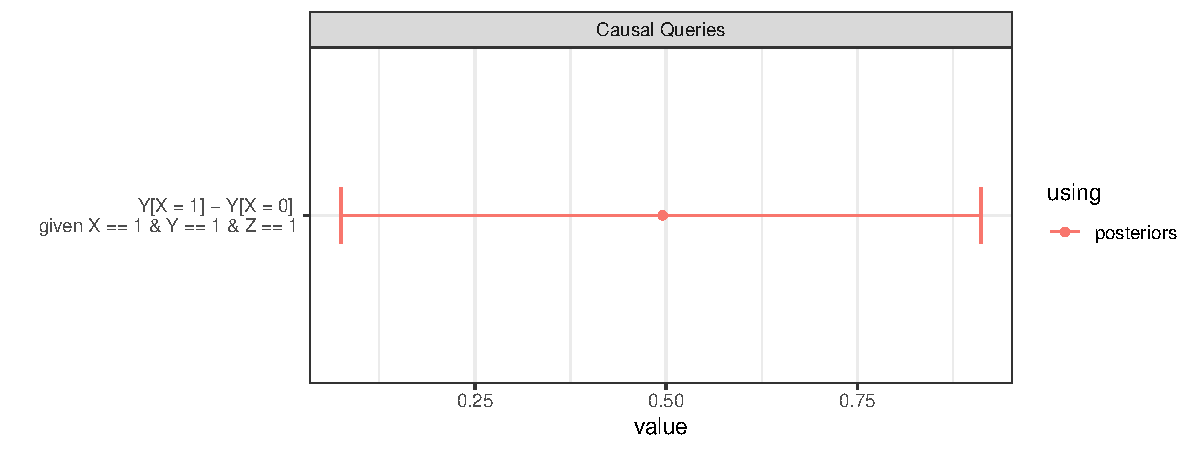
\includegraphics[keepaspectratio]{paper_files/figure-pdf/fig-case-level-query-1.pdf}}

}

\caption{\label{fig-case-level-query}Illustration of case-level queries
plotted.}

\end{figure}%

The result in Figure~\ref{fig-case-level-query} is what we should now
believe for all cases in which \(Z=1\), \(X=1\), and \(Y=1\). It is the
expected average effect among cases with this data type, so this
expectation has an uncertainty attached to it, reflecting our
uncertainty about the expectation.

This can differ, however, from what we would infer if we were presented
with a new case drawn from the population. When examining a new case, we
must \emph{update} based on the information provided about that case.
This \emph{new} case-level inference is calculated when the
\texttt{case\_level\ =\ TRUE} argument is specified. For a query \(Q\)
and given \(D\), this returns the value
\(\frac{\int\pi(Q \& D | \lambda_i)p(\lambda_i)d\lambda_i}{\int\pi(D | \lambda_i)p(\lambda_i)d\lambda_i}\),
which may differ from the mean of the distribution
\(\frac{\pi(Q \& D | \lambda)}{\pi(D | \lambda)}\) given by
\(\int \frac{\pi(Q \& D | \lambda_i)}{\pi(D | \lambda_i)} p(\lambda_i)d\lambda_i\).

To illustrate the difference, consider an
\(X \rightarrow M \rightarrow Y\) model where we are quite certain that
\(X\) causes \(Y\), but unsure whether this effect works through two
positive or two negative effects. If asked what we would think about
effects in cases \(M=0\) (or with \(M=1\)), we have little basis to know
whether these are cases in which effects are more or less likely.
However, if we randomly find a case and we observe that \(M=0\), our
understanding of the causal model evolves, leading us to believe there
is (or is not) an effect in this specific case. The case-level query
gives a single value without posterior standard deviation, representing
the belief about this new case.

\begin{CodeInput}
R> make_model("X -> M -> Y") |> update_model(
+    data.frame(X = rep(0:1, 8), Y = rep(0:1, 8)), iter = 4000, refresh = 0) |>
+    query_model("Y[X = 1] > Y[X = 0] :|: X == 1 & Y == 1 & M == 1", 
+    using = "posteriors", case_level = c(TRUE, FALSE)) |>
+    plot()
\end{CodeInput}

\begin{figure}[H]

\centering{

\pandocbounded{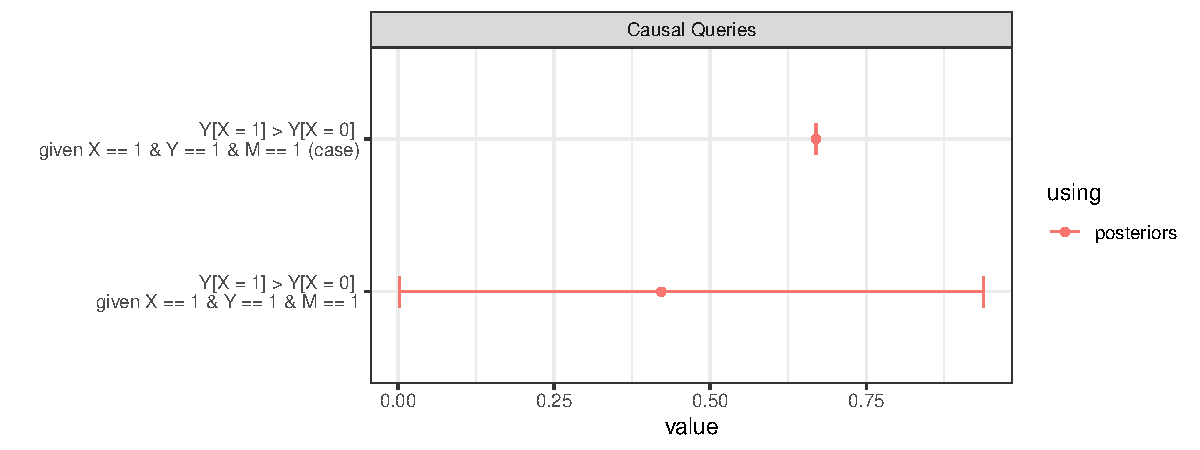
\includegraphics[keepaspectratio]{paper_files/figure-pdf/fig-new-case-level-query-1.pdf}}

}

\caption{\label{fig-new-case-level-query}Illustration of new case-level
queries plotted.}

\end{figure}%

\subsubsection{Batch queries}\label{batch-queries}

The function \texttt{query\_model()} can also be used to pose multiple
queries of multiple models in batch. The function takes a list of
models, causal queries, and conditions as inputs. It then calculates
population or case level estimands given prior or posterior
distributions and reports summaries of these distributions. The result
is a data frame of class \texttt{model\_query} (see
Section~\ref{sec-classes}) that can be displayed as a table or used for
graphing. The associated \texttt{plot} method produces plots with class
\texttt{c("gg",\ "ggplot")}.

Since users can adjust multiple lists of features of a query there is an
option, \texttt{expand\_grid\ =\ TRUE}, to indicate whether to query
with respect to all combinations of supplied arguments.

To illustrate, we return again to the lipids model but now consider two
versions, one with and one without a monotonicity restriction imposed.

\begin{CodeInput}
R> models <- list(
+    Unrestricted = lipids_model |> 
+    update_model(data = lipids_data, refresh = 0),
+    Restricted = lipids_model |> set_restrictions("X[Z = 1] < X[Z = 0]") |> 
+    update_model(data = lipids_data, refresh = 0)
+    )
\end{CodeInput}

Table~\ref{tbl-batch-query} then shows the output from a single call to
\texttt{query\_model()} with the \texttt{expand\_grid} argument set to
\texttt{TRUE} to generate all combinations of list elements.

\begin{CodeInput}
R> queries <- 
R> query_model(
+    models, 
+    query = list(
+    ATE = "Y[X=1] - Y[X=0]", 
+    POS = "Y[X=1] > Y[X=0] :|: Y==1 & X==1"),
+    case_level = c(FALSE, TRUE), 
+    using = c("priors", "posteriors"),
+    expand_grid = TRUE)
\end{CodeInput}

\begin{longtable}{ccccccc}

\toprule
label & model & query & given & using & case\_level & mean\\
\midrule
ATE & Unrestricted & Y[X=1] - Y[X=0] & - & priors & FALSE & 0.00\\
ATE & Restricted & Y[X=1] - Y[X=0] & - & priors & FALSE & 0.00\\
ATE & Unrestricted & Y[X=1] - Y[X=0] & - & posteriors & FALSE & 0.56\\
ATE & Restricted & Y[X=1] - Y[X=0] & - & posteriors & FALSE & 0.55\\
POS & Unrestricted & Y[X=1] > Y[X=0] & Y==1 \& X==1 & priors & FALSE & 0.50\\
POS & Restricted & Y[X=1] > Y[X=0] & Y==1 \& X==1 & priors & FALSE & 0.49\\
POS & Unrestricted & Y[X=1] > Y[X=0] & Y==1 \& X==1 & posteriors & FALSE & 0.95\\
POS & Restricted & Y[X=1] > Y[X=0] & Y==1 \& X==1 & posteriors & FALSE & 0.95\\
ATE & Unrestricted & Y[X=1] - Y[X=0] & - & priors & TRUE & 0.00\\
ATE & Restricted & Y[X=1] - Y[X=0] & - & priors & TRUE & 0.00\\
ATE & Unrestricted & Y[X=1] - Y[X=0] & - & posteriors & TRUE & 0.56\\
ATE & Restricted & Y[X=1] - Y[X=0] & - & posteriors & TRUE & 0.55\\
POS & Unrestricted & Y[X=1] > Y[X=0] & Y==1 \& X==1 & priors & TRUE & 0.50\\
POS & Restricted & Y[X=1] > Y[X=0] & Y==1 \& X==1 & priors & TRUE & 0.49\\
POS & Unrestricted & Y[X=1] > Y[X=0] & Y==1 \& X==1 & posteriors & TRUE & 0.95\\
POS & Restricted & Y[X=1] > Y[X=0] & Y==1 \& X==1 & posteriors & TRUE & 0.95\\
\bottomrule


\caption{\label{tbl-batch-query}Results for two queries on two models.}

\tabularnewline
\end{longtable}

Figure~\ref{fig-batch} shows the default plot associated with this
query.

\begin{figure}

\centering{

\pandocbounded{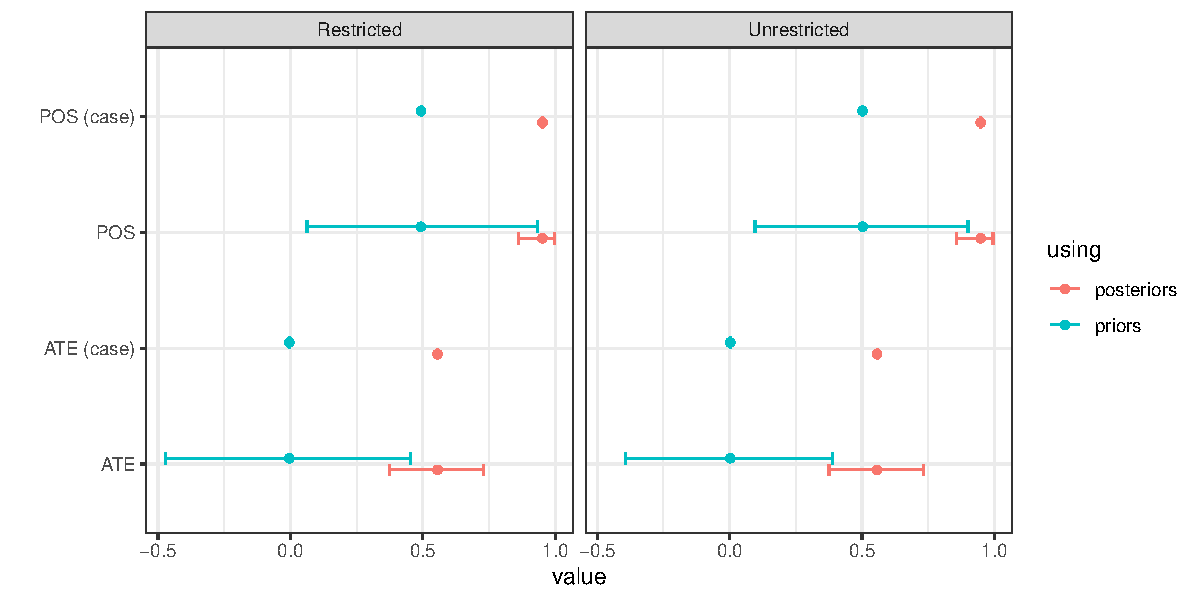
\includegraphics[keepaspectratio]{paper_files/figure-pdf/fig-batch-1.pdf}}

}

\caption{\label{fig-batch}Default plotting for a a set of queries over
multiple models.}

\end{figure}%

\section{Summary and discussion}\label{summary-and-discussion}

\pkg{CausalQueries} provides an intuitive user interface to generate,
update, and query causal models defined over binary nodes.

A particular strength is the flexibility users enjoy in specifying the
structure of causal models and querying them using an integrated
framework. Rather than requiring bespoke functions for different types
of problems---studying treatment effects in randomized experiments,
complier effects in encouragement designs, or mediation quantities in
more complex causal structures---a unified procedure is used for
defining models and for updating on model parameters. With updated
models in hand, queries involving arbitrary \(do\) operations can be
posed using an intuitive syntax.

We identify several areas for future expansion of the package's
functionality. One area involves extending the class of models that can
be passed to \texttt{make\_model()} to accommodate non-binary data and
hierarchical data structures. Proofs of concept for both extensions are
available in \citet{humphreys_integrated_2023}. Inspired by new work in
\citet{irons2023causally}, we see potential in allowing the
specification of more flexible prior distributions and developing
algorithms for faster updating in these settings. Inspired by conditions
for identification of mediation quantities in
\citet{forastiere2018principal}, we see potential for allowing more
flexible constraints over the joint distribution of nodal types. For
querying, we see scope for facilitating nonlinear complex causal
queries, such as risk ratios, which currently require combining multiple
simple causal queries. Finally, we see potential for more integrated
functionality for model validation, including assessments of the
sensitivity of conclusions to priors.

\FloatBarrier

\newpage{}

\section*{Computational details and software
requirements}\label{computational-details-and-software-requirements}
\addcontentsline{toc}{section}{Computational details and software
requirements}

\begin{longtable}[]{@{}
  >{\raggedright\arraybackslash}p{(\linewidth - 4\tabcolsep) * \real{0.1800}}
  >{\raggedright\arraybackslash}p{(\linewidth - 4\tabcolsep) * \real{0.4100}}
  >{\raggedright\arraybackslash}p{(\linewidth - 4\tabcolsep) * \real{0.4100}}@{}}
\toprule\noalign{}
\endhead
\bottomrule\noalign{}
\endlastfoot
Version & \begin{minipage}[t]{\linewidth}\raggedright
\begin{itemize}
\tightlist
\item
  1.4.3
\end{itemize}
\end{minipage} & \\
Availability & \begin{minipage}[t]{\linewidth}\raggedright
\begin{itemize}
\tightlist
\item
  Stable Release:
  \url{https://cran.rstudio.com/web/packages/CausalQueries/index.html}
\item
  Development:
  \url{https://github.com/integrated-inferences/CausalQueries}
\end{itemize}
\end{minipage} & \\
Issues & \begin{minipage}[t]{\linewidth}\raggedright
\begin{itemize}
\tightlist
\item
  \url{https://github.com/integrated-inferences/CausalQueries/issues}
\end{itemize}
\end{minipage} & \\
Operating Systems & \begin{minipage}[t]{\linewidth}\raggedright
\begin{itemize}
\tightlist
\item
  Linux
\item
  MacOS
\item
  Windows
\end{itemize}
\end{minipage} & \\
Testing Environments OS & \begin{minipage}[t]{\linewidth}\raggedright
\begin{itemize}
\tightlist
\item
  Ubuntu 22.04.2
\item
  Debian 12.2
\item
  MacOS
\item
  Windows
\end{itemize}
\end{minipage} & \\
Testing Environments R & \begin{minipage}[t]{\linewidth}\raggedright
\begin{itemize}
\tightlist
\item
  R 4.4.2
\item
  R 4.3.3
\item
  R 4.2.3
\item
  r-devel
\end{itemize}
\end{minipage} & \\
R Version & \begin{minipage}[t]{\linewidth}\raggedright
\begin{itemize}
\tightlist
\item
  R(\textgreater= 4.2.0)
\end{itemize}
\end{minipage} & \\
Compiler & \begin{minipage}[t]{\linewidth}\raggedright
\begin{itemize}
\tightlist
\item
  either of the below or similar:
\item
  g++
\item
  clang++
\end{itemize}
\end{minipage} & \\
Stan requirements & \begin{minipage}[t]{\linewidth}\raggedright
\begin{itemize}
\tightlist
\item
  inline
\item
  RcppEigen (\textgreater= 0.3.3.3.0)
\item
  RcppArmadillo (\textgreater= 0.12.6.4.0)
\item
  RcppParallel (\textgreater= 5.1.4)
\item
  BH (\textgreater= 1.66.0)
\item
  StanHeaders (\textgreater= 2.26.0)
\item
  rstan (\textgreater= 2.26.0)
\end{itemize}
\end{minipage} & \\
R-Packages Depends & \begin{minipage}[t]{\linewidth}\raggedright
\begin{itemize}
\tightlist
\item
  methods
\end{itemize}
\end{minipage} & \\
R-Packages Imports & \begin{minipage}[t]{\linewidth}\raggedright
\begin{itemize}
\tightlist
\item
  dirmult (\textgreater= 0.1.3-4) \textbar{}
\item
  dplyr \textbar{}
\item
  stats (\textgreater= 4.1.1) \textbar{}
\item
  rlang (\textgreater= 0.2.0) \textbar{}
\item
  rstan (\textgreater= 2.26.0) \textbar{}
\item
  rstantools (\textgreater= 2.0.0) \textbar{}
\item
  stringr (\textgreater= 1.4.0) \textbar{}
\item
  latex2exp (\textgreater= 0.9.4) \textbar{}
\item
  knitr (\textgreater= 1.45) \textbar{}
\item
  ggplot2 (\textgreater= 3.3.5) \textbar{}
\item
  lifecycle (\textgreater= 1.0.1) \textbar{}
\item
  ggraph (\textgreater= 2.2.0) \textbar{}
\item
  Rcpp (\textgreater= 0.12.0) \textbar{}
\end{itemize}
\end{minipage} & \\
\end{longtable}

Computational details and software requirements.

The results in this paper were obtained using
\proglang{R}\textasciitilde4.3 with the \pkg{MASS}\textasciitilde7.3-60
package. \proglang{R} itself and all packages used are available from
the Comprehensive \proglang{R} Archive Network (CRAN) at
\url{https://CRAN.R-project.org/}.

\section*{Acknowledgments}\label{acknowledgments}
\addcontentsline{toc}{section}{Acknowledgments}

\begin{tcolorbox}[enhanced jigsaw, colback=white, rightrule=.15mm, toprule=.15mm, left=2mm, bottomrule=.15mm, breakable, arc=.35mm, leftrule=.75mm, colframe=quarto-callout-color-frame, opacityback=0]

We thank Ben Goodrich, who provided generous insights on using
\texttt{stan} for this project. We thank Alan M Jacobs for key work in
developing the framework underlying the package. Our thanks to
Cristian-Liviu Nicolescu, who provided wonderful feedback on the use of
the package and a draft of this paper. Our thanks to Jasper Cooper for
contributions to the generic function to create Stan code, to
\href{https://clarabicalho.github.io/}{Clara Bicalho}, who helped figure
out the syntax for causal statements, to
\href{https://www.gov.harvard.edu/directory/julio-s-solis-arce/}{Julio
S. Solís Arce} who made many vital contributions figuring out how to
simplify the specification of priors, and to
\href{https://merlinheidemanns.github.io/website/}{Merlin Heidemanns}
who figured out the \texttt{rstantools} integration and made myriad code
improvements.

\end{tcolorbox}

\section*{References}\label{references}
\addcontentsline{toc}{section}{References}

\renewcommand{\bibsection}{}
\bibliography{supp/cq_jss.bib}

\newpage{}

\section*{Appendix A: Parallelization}\label{sec-parallel}
\addcontentsline{toc}{section}{Appendix A: Parallelization}

If users have access to multiple cores, parallel processing can be
implemented by including this line before running \pkg{CausalQueries}:

Additionally, parallelizing across models or data while running MCMC
chains in parallel can be achieved by setting up a nested parallel
process. With 8 cores one can run two updating processes with three
parallel chains each simultaneously. More generally the number of
parallel processes at the upper level of the nested parallel structure
are given by \(\left \lfloor \frac{cores}{chains + 1} \right \rfloor\).

\begin{CodeInput}
R> library("future")
R> library("future.apply")
R> chains <- 3
R> cores <- 8
R> future::plan(list(
+    future::tweak(future::multisession, 
+    workers = floor(cores/(chains + 1))),
+    future::tweak(future::multisession, workers = chains)))
R> model <- make_model("X -> Y")
R> data <- list(data_1 = data.frame(X = 0:1, Y = 0:1), 
+    data_2 = data.frame(X = 0:1, Y = 1:0))
R> results <- future.apply::future_lapply(data, function(d) {
+    update_model(model = model, data = d, chains = chains, refresh = 0)},
+    future.seed = TRUE)
\end{CodeInput}

\newpage{}

\section*{Appendix B: Stan code}\label{sec-stancode}
\addcontentsline{toc}{section}{Appendix B: Stan code}

Updating is performed using a generic Stan model. The data provided to
Stan is generated by the internal function \texttt{prep\_stan\_data()},
which returns a list of objects that Stan expects to receive. The code
for the Stan model is shown below. After defining a helper function, the
code starts with a block declaring what input data is to be expected.
Then, the parameters and the transformed parameters are characterized.
Then, the likelihoods and priors are provided. At the end, a block for
generated quantities is used to append a posterior distribution of
causal types to the model.

\begin{verbatim}
S4 class stanmodel 'simplexes' coded as follows:
functions {
  row_vector col_sums(matrix X) {
    row_vector[cols(X)] s;
    s = rep_row_vector(1, rows(X)) * X;
    return s;
  }
}
data {
  int<lower=1> n_params;
  int<lower=1> n_paths;
  int<lower=1> n_types;
  int<lower=1> n_param_sets;
  int<lower=1> n_nodes;
  array[n_param_sets] int<lower=1> n_param_each;
  int<lower=1> n_data;
  int<lower=1> n_events;
  int<lower=1> n_strategies;
  int<lower=0, upper=1> keep_type_distribution;
  vector<lower=0>[n_params] lambdas_prior;
  array[n_param_sets] int<lower=1> l_starts;
  array[n_param_sets] int<lower=1> l_ends;
  array[n_nodes] int<lower=1> node_starts;
  array[n_nodes] int<lower=1> node_ends;
  array[n_strategies] int<lower=1> strategy_starts;
  array[n_strategies] int<lower=1> strategy_ends;
  matrix[n_params, n_types] P;
  matrix[n_params, n_paths] parmap;
  matrix[n_paths, n_data] map;
  matrix<lower=0, upper=1>[n_events, n_data] E;
  array[n_events] int<lower=0> Y;
}
parameters {
  vector<lower=0>[n_params - n_param_sets] gamma;
}
transformed parameters {
  vector<lower=0, upper=1>[n_params] lambdas;
  vector<lower=1>[n_param_sets] sum_gammas;
  matrix[n_params, n_paths] parlam;
  matrix[n_nodes, n_paths] parlam2;
  vector<lower=0, upper=1>[n_paths] w_0;
  vector<lower=0, upper=1>[n_data] w;
  vector<lower=0, upper=1>[n_events] w_full;
  vector[n_param_sets] log_sum_gammas;
  // Handle cases where parameter set has only one value
  for (i in 1:n_param_sets) {
    if (l_starts[i] >= l_ends[i]) {
      sum_gammas[i] = 1;
      lambdas[l_starts[i]] = 1;
    } else {
      sum_gammas[i] = 1 + sum(gamma[(l_starts[i] - (i - 1)):(l_ends[i] - i)]);
      lambdas[l_starts[i]:l_ends[i]] =
        append_row(1, gamma[(l_starts[i] - (i - 1)):(l_ends[i] - i)]) /
        sum_gammas[i];
    }
  }
  // Mapping from parameters to data types
  parlam = rep_matrix(lambdas, n_paths) .* parmap;
  // Sum probability over nodes on each path
  for (i in 1:n_nodes) {
    parlam2[i, ] = col_sums(parlam[(node_starts[i]):(node_ends[i]), ]);
  }
  // Compute probability of data type on each path
  for (i in 1:n_paths) {
    w_0[i] = exp(sum(log(parlam2[, i])));
  }
  // Map to n_data columns instead of n_paths (if confounding)
  w = map' * w_0;
  // Extend/reduce to cover all observed data types
  w_full = E * w;
  // Calculate log sum gammas once for efficiency
  log_sum_gammas = log(sum_gammas);
}
model {
  // Dirichlet distributions
  for (i in 1:n_param_sets) {
    target += dirichlet_lpdf(lambdas[l_starts[i]:l_ends[i]] |
                             lambdas_prior[l_starts[i]:l_ends[i]]);
    target += -n_param_each[i] * log_sum_gammas[i];
  }
  // Multinomial likelihoods (handling censoring)
  for (i in 1:n_strategies) {
    target += multinomial_lpmf(
      Y[strategy_starts[i]:strategy_ends[i]] |
      w_full[strategy_starts[i]:strategy_ends[i]] /
      sum(w_full[strategy_starts[i]:strategy_ends[i]])
    );
  }
}
// Option to export distribution of causal types
generated quantities {
  vector[n_types] types;
  if (keep_type_distribution == 1) {
    for (i in 1:n_types) {
      types[i] = prod(P[, i] .* lambdas + 1 - P[, i]);
    }
  } else {
    types = rep_vector(1, n_types);
  }
} 
\end{verbatim}

\newpage{}

\section*{Appendix C: Benchmarks}\label{sec-benchmark}
\addcontentsline{toc}{section}{Appendix C: Benchmarks}

We present a brief summary of model updating benchmarks. Note that these
benchmarks are not generally reproducible and depend on the
specifications of the hardware system used to produce them. The first
benchmark considers the effect of model complexity on updating time. The
second benchmark considers the effect of data size on updating time. We
run four parallel chains for each model with a relatively large number
(4000) of iterations each time, all replicated five times. The results
of the benchmarks are presented in Table~\ref{tbl-bench1} and
Table~\ref{tbl-bench2}.

Increasing the number of parents in a model greatly increases the number
of parameters and computational time. The results suggests the
computational time is convex in the number of parents. Unless model
restrictions are imposed, four parents would yield 65,536 parameters.
The rapid growth of the parameter space with increasing model complexity
places limits on feasible computability without further recourse to
specialized methods for handling large causal models. In contrast, the
results suggest that computational time is concave in the size of the
data.

\begin{longtable}{ccc}

\toprule
Model & Number of parameters & Runtime (seconds)\\
\midrule
X1 → Y & 6 & 934.35\\
X1 → Y; X2 → Y & 20 & 2152.34\\
X1 → Y; X2 → Y; X3 → Y & 262 & 50556.00\\
\bottomrule


\caption{\label{tbl-bench1}Benchmarking 1.}

\tabularnewline
\end{longtable}

\begin{longtable}{ccc}

\toprule
Model & Number of observations & Runtime (seconds)\\
\midrule
X1 → Y & 10 & 724.55\\
X1 → Y & 100 & 791.52\\
X1 → Y & 1000 & 1629.63\\
X1 → Y & 10000 & 3743.58\\
\bottomrule


\caption{\label{tbl-bench2}Benchmarking 2.}

\tabularnewline
\end{longtable}

\newpage{}





\end{document}
